\documentclass[11pt]{article}
\usepackage[margin=1in]{geometry}
\usepackage[T1]{fontenc}
\usepackage{lmodern}
\usepackage{microtype}
\usepackage{booktabs}
\usepackage{amsmath,amssymb}
\usepackage{graphicx}
\usepackage{hyperref}
\usepackage[numbers,sort&compress]{natbib}
\usepackage{caption}
\captionsetup{font=small}

\title{Cross-Dataset Network Intrusion Detection: Why Transfer Fails and What a Few Target Labels Can Recover}
\author{Quang-Vinh Dang\\
British University Vietnam, Hung Yen, Vietnam\\
\texttt{vinh.dq4@buv.edu.vn}\quad ORCID 0000-0002-3877-8024}
\date{}

\begin{document}
\maketitle

\begin{abstract}
Machine-learning detectors of malicious network flows reach 0.985 ROC-AUC when trained and tested on one dataset and then lose most of that skill on another network.
We build a benchmark of seven public flow datasets from five laboratories and three flow extractors, harmonised to 13 features of the same physical meaning, and evaluate eight baselines and nine variants of a domain-invariant method of our own, RIFT (Rank-Invariant Flow Transfer), in 42 ordered source--target transfers and seven leave-one-dataset-out tasks over three seeds.
Tree ensembles reach 0.54 to 0.56 ROC-AUC across transfers, 36 to 48\% of the transfers are below chance, and RIFT is below its own boosting baseline (0.484 against 0.557), even when it is given the true target prior (0.488) or a reference set of truly benign flows (0.543).
Transfer of a single attack family between datasets is also near chance (median 0.545 over 74 dataset--family cells), which excludes a difference of attack mix alone; our controls cannot separate differences in benign traffic, in measurement and in the conditional label distribution.
We then ask what the other datasets can still contribute when only $k=4$ to $128$ target flows are labelled.
We meta-train a transformer, FLARE-2 (Few-shot Learning of Attack Rules across Environments), on tasks from the other datasets and compare it with tree ensembles and with TabPFN versions 3 and 3.5, general-purpose tabular foundation models that we did not train or tune on network data.
Over eight targets and three meta-training seeds, FLARE-2 shows no significant difference from random forest and CatBoost on binary ROC-AUC ($+0.001$ and $-0.001$), but TabPFN-3.5 is higher than FLARE-2 on every target (mean difference $-0.014$, 95\% interval $[-0.018,-0.011]$); at attack-class level the two have similar per-class ROC-AUC ($-0.002$) and TabPFN-3.5 has higher recall.
In our experiments, meta-training on real network tasks therefore did not improve on a general-purpose pretrained prior.
Code and all raw results are public.
\end{abstract}

\section{Introduction}
Flow-based network intrusion detection is usually evaluated by splitting one dataset into a training and a test part.
Under that protocol gradient-boosted trees exceed 0.99 ROC-AUC on CIC-IDS2017 and USB-IDS-1 (ROC-AUC is the probability that a detector scores a randomly chosen attack flow above a randomly chosen benign flow: 1 is perfect, 0.5 is chance, and values below 0.5 mean that the detector ranks attacks as \emph{less} suspicious than benign traffic).
A growing literature shows that the same models degrade sharply on a second dataset \citep{layeghy2023explainable,cantone2024crossdataset,dhooge2020inter,dhooge2023damaged,apruzzese2022cross}, and even datasets from one laboratory transfer poorly.
Two explanations are common.
The first is covariate shift: capture tools, link speeds and traffic mixes change the scale and distribution of features, which normalisation or domain adaptation could repair \citep{ganin2016dann,sun2016coral,layeghy2023dinids}.
The second is that the datasets define attacks differently, so that the same flow statistics carry different labels, which no unlabelled adaptation can repair.

This paper asks two questions.
\emph{Why does transfer fail?} We build a benchmark, design a domain-invariant method (RIFT, Sect.~\ref{sec:rift}) to repair the shifts that the first explanation names, and run controls that narrow down the explanation.
\emph{What can other datasets still contribute when a few target flows are labelled?} We meta-train a transformer on tasks from the other datasets (that is, we train it on many small classification tasks so that it can learn a new task from a few labelled examples) and compare it with tree ensembles and with a general-purpose tabular foundation model (a model pretrained on a very large collection of tabular tasks, which we apply without training on our data).
We make four contributions.
\begin{enumerate}
\item \textbf{A benchmark} of seven public datasets (an eighth, CTU-13, supports only a minimal feature tier and is used in the few-label study; Table~\ref{tab:datasets}) with a common flow schema, a bottom-$k$ hash sampler that gives a reproducible uniform sample of distinct rows, and a protocol with in-domain, pairwise (42 ordered pairs, labelled by whether the pair shares a laboratory or an extractor) and leave-one-dataset-out (LODO) settings, in inductive and transductive modes, over three seeds.
\item \textbf{A method designed to work, and its failure, with controls.} RIFT replaces each feature by its rank within its own dataset so that scales no longer matter, aligns the target's benign traffic with the sources' using flows estimated to be benign, keeps only features whose relation to the label has the same sign in every source, and corrects the output for the different share of attacks in the target. A full ablation and two oracle diagnostics show that it is below its own baseline and that supplying the information it estimates does not fix it. Controls (an oracle search, single-attack-family transfer, a nearest-neighbour test, per-feature signs, dataset identity, a few-label comparison) narrow down the explanation, and Table~\ref{tab:controls} states what each can and cannot show.
\item \textbf{FLARE-2} (Few-shot Learning of Attack Rules across Environments), a few-label meta-learner for flow data trained on tasks from other networks. It is permutation-invariant over features, accepts any feature set, and handles binary detection and attack-type classification with the same readout.
\item \textbf{A comparison with a tabular foundation model, which is the main finding for the second question.} TabPFN versions 3 and 3.5, general-purpose transformers that classify new rows by reading labelled examples given as input, and that we did not train or tune on network data (the model card of version 3 states that it is trained purely on synthetic tabular tasks \citep{priorlabs2026tabpfn3}), are better than FLARE-2 on binary ROC-AUC on every target (mean over $k$) by 0.008 (TabPFN-3, seed 0) to 0.014 (TabPFN-3.5, three seeds), and TabPFN-3.5 is above random forest on all targets. The evaluation uses the target dataset as the unit of analysis, exact Wilcoxon tests, bootstrap intervals, three meta-training seeds and controls for normalisation and in-context behaviour.
\end{enumerate}
We do not claim that FLARE-2 is the best few-label method: it matches fixed-setting tree ensembles on binary ROC-AUC and a general-purpose foundation model is better.
What the study supports is that a few labelled flows of the target network, combined with a strong pretrained prior, are the reliable ingredient, and that, in our experiments, meta-training on real network tasks did not improve on that prior at the binary level.

\section{Related work}
\paragraph{Machine learning for intrusion detection.}
Learning-based detection of malicious network traffic has been studied for decades, and comparisons of learning algorithms, feature sets and training regimes fill the literature.
Our earlier work studied machine-learning techniques for intrusion detection systems in general \citep{dang2019studying,dang2022cai,dang2022mlids} and applied them to named datasets and environments: CIDDS-001 \citep{dang2021cidds,dang2022cidds}, USB-IDS-1 \citep{dang2023usbmulti}, software-defined networks \citep{dang2021sdn,dang2024fuzzy}, DNS attacks \citep{dang2022dns,dang2021fuzzydns}, WiFi networks \citep{dang2023wifi} and medical Internet-of-Things traffic \citep{dang2024iomt}.
The same line of work examined the explanation of detector decisions and its relation to detection performance \citep{dang2020understand,dang2021explain}, active learning \citep{dang2020active} and reinforcement learning \citep{dang2022rl} for the task.
Newer model families have also been applied to intrusion detection in our own studies: transformers \citep{dang2023transformer}, graph neural networks \citep{dang2023wifi}, embeddings from large language models \citep{dang2025llm}, fuzzy embeddings \citep{dang2024fuzzy}, kernel methods for conformal prediction and uncertainty measures \citep{dang2024conformal,dang2026uncertainty}, parallel optimisation for lightweight detectors \citep{dang2024lightweight} and federated explainable detectors \citep{dang2026stfedxids}.
Most of these concern a single named dataset or environment; how a detector trained on one network behaves on another is the subject of the cross-dataset work below.

\paragraph{Datasets and evaluation practice.}
The datasets are themselves the subject of surveys: \citet{ashraf2026survey} examine 124 datasets for intrusion detection in communication networks and report critical gaps such as limited real-world traffic representation, inconsistent documentation, dataset bias and evaluation risks.
The datasets used here come from different laboratories and extractors: CIC-IDS2017 \citep{sharafaldin2018cicids} and CIC-IDS2018, USB-IDS-1 \citep{catillo2021usbids1,catillo2025usbidstc}, InSDN \citep{elsayed2020insdn}, UNSW-NB15 \citep{moustafa2015unsw}, ToN-IoT \citep{alsaedi2020toniot}, IoT-23 \citep{garcia2020iot23} and CTU-13 \citep{garcia2014ctu13}.
\citet{engelen2021troubleshooting} document flow-construction and labelling errors in CIC-IDS2017, \citet{arp2022dos} discuss pitfalls of machine learning in security, among them sampling bias, spurious correlations and evaluation in the laboratory only, and \citet{apruzzese2023sok} survey assessment practices.
\citet{sarhan2021netflow,sarhan2022standard,sarhan2022evaluating} build NetFlow versions of several datasets and propose standard NetFlow feature sets to increase the generalisability of detectors, and \citet{alriyami2021cross} show on NSL-KDD and gureKDD that a cross-dataset collapse can be caused by a mismatch of feature definitions between datasets, which is a caution for any study that merges feature schemas, including ours.

\paragraph{Cross-dataset generalisation.}
\citet{layeghy2023explainable} train on one NetFlow-v2 dataset and test on another and report attack-class F1 below 1\% for several pairs of CIC-IDS2018, UNSW-NB15 and ToN-IoT, with strongly asymmetric results that they attribute, with SHAP feature attributions, to features that correlate with the label in only one dataset; a domain-invariance method of the same group \citep{layeghy2023dinids} improves some pairs.
\citet{cantone2024crossdataset} report a Matthews correlation coefficient (MCC, a chance-corrected score from $-1$ to $1$) between 0.26 and 0.44 when CIC-IDS2017 and CIC-IDS2018 are exchanged, even though both come from the same laboratory, and \citet{kilic2026shap} report a macro-F1 between about 0.12 and 0.21 between the same two datasets, with and without SHAP-based feature reduction.
\citet{dhooge2020inter,dhooge2023damaged} analyse inter-dataset generalisation per attack class and the effect of data-damaged models on it, \citet{catillo2022transferability} study transfer from CIC-IDS2017 to USB-IDS-1 \citep{catillo2021usbids1}, which share an extractor, \citet{apruzzese2022cross} cross-evaluate per-attack detectors across several networks, and \citet{hossain2026assessing} test UNSW-NB15 and ToN-IoT on seven shared features.
Our own earlier work addressed the same problem for software-defined networks, where models that perform well within one dataset lose performance when the test data are collected from another source, and applied concept-drift detection techniques to improve the cross-dataset performance \citep{dang2023learning}; another study used several datasets of software-defined networks to detect intrusion \citep{dang2022multisdn}.
The present benchmark differs in covering seven datasets and three extractors with one schema, in labelling each pair by how much infrastructure the two datasets share, in running label-free transfer methods against default-setting baselines over three seeds, and in reporting the controls that decide whether the negative result is a finding.

\paragraph{Domain adaptation, invariance and label shift.}
Domain-adversarial training \citep{ganin2016dann} and correlation alignment \citep{sun2016coral} align source and target feature distributions without target labels, and the domain-invariance detector of \citet{layeghy2023dinids} builds on adversarial alignment.
They assume that the labelling function is shared between the domains, and the expectation-maximisation correction of the output prior of \citet{saerens2002adjusting}, which RIFT uses, assumes pure label shift.
Our controls probe these assumptions but cannot isolate concept shift from a change of attack mix, and we evaluate the methods against their own baselines in the same setting.

\paragraph{Few-shot, meta-learning and in-context learning.}
Matching and prototypical networks \citep{vinyals2016matching,snell2017prototypical} and gradient-based meta-learning \citep{finn2017maml} learn from episodes.
Prior-fitted networks \citep{muller2022pfn} and TabPFN \citep{hollmann2025tabpfn} fit a transformer to synthetic tabular tasks and classify by attention to the labelled rows; later versions of TabPFN are distributed with their own model cards \citep{priorlabs2026tabpfn3}.
FLARE-2 follows this in-context recipe but meta-trains on \emph{real} tasks from other networks, adds a task distribution designed for the cross-network case, and uses a matching readout that fits a variable label space; set-based architectures \citep{lee2019settransformer} motivate its permutation invariance over rows and features.
We also evaluate TabPFN itself, versions 3 and 3.5, on the same supports, which tests whether meta-training on network tasks adds anything to a model pretrained on synthetic tasks only, and we compare with gradient-boosted trees \citep{prokhorenkova2018catboost}.

\paragraph{What is missing, and what we do.}
The studies above leave three gaps that motivate this paper.
First, the cross-dataset studies evaluate two to four datasets, each with its own feature set and metric (F1, MCC, balanced accuracy), so one favourable or unfavourable pair can dominate the picture and the numbers cannot be compared across studies.
Second, a positive or a negative result is hard to interpret without controls that show whether it reflects the data or the implementation and tuning of the method, and such controls are rarely reported together with the result.
Third, a defender who can label a few flows of the new network needs to know what source data can still add and how that compares with modern pretrained tabular models; the few-label setting has been studied less and, to our knowledge, not against such models on flow datasets.
We address the gaps in turn.
Section~\ref{sec:bench} builds a benchmark with one schema and one protocol for seven datasets and defines the methods that we compare, among them a domain-invariant method of our own.
Section~\ref{sec:results} uses it to show that transfer fails, tests whether that method repairs it, and runs controls that narrow down the explanation.
Section~\ref{sec:fewlabel} then turns to the few-label setting and compares a meta-trained transformer with trees and with a tabular foundation model, and Sect.~\ref{sec:disc} discusses what the evidence does and does not show.

\section{Benchmark and methods}\label{sec:bench}
This section describes the benchmark (Sect.~\ref{sec:benchdata}) and the methods that we compare (Sect.~\ref{sec:benchmeth} and~\ref{sec:rift}).
Table~\ref{tab:terms} explains the terms and abbreviations used in the rest of the paper.

\begin{table}[t]
\centering\small
\caption{Terms and abbreviations.}\label{tab:terms}
\begin{tabular}{p{0.2\textwidth}p{0.72\textwidth}}
\toprule
Term & Meaning \\
\midrule
Source, target & The dataset(s) a model is trained on, and the dataset it is tested on. \\
Pairwise transfer & Train on one source dataset, test on one other dataset (42 ordered pairs of seven datasets). \\
LODO & Leave-one-dataset-out: train on all other datasets pooled, test on the held-out one. \\
Inductive, transductive & Inductive: the method sees nothing from the target. Transductive: it also sees the target's unlabelled features. \\
Label-free, few-label & Label-free: no target label is used. Few-label: $k$ labelled target flows are available ($k=4$ to 128). \\
ROC-AUC & Probability that a random attack flow is scored above a random benign flow; 1 perfect, 0.5 chance. \\
MCC, F1, FPR & Matthews correlation coefficient; F1 score; false-positive rate (share of benign flows flagged as attacks). Recall is the share of attacks detected. \\
LR, RF & Logistic regression; random forest (an ensemble of decision trees). \\
HGB & Histogram-based gradient boosting: gradient-boosted decision trees whose feature values are binned into histograms for speed (scikit-learn \texttt{HistGradientBoostingClassifier}). It is the reference classifier of the benchmark and the classifier inside RIFT. \\
CatBoost, XGBoost & Two other libraries for gradient-boosted decision trees. \\
MLP & Multi-layer perceptron, a small feed-forward neural network. \\
CORAL & Correlation alignment: re-colours the source features so that their covariance matches the target's, then trains a classifier. \\
DANN & Domain-adversarial neural network: a classifier whose internal features are trained so that a second network cannot tell source from target. \\
RIFT & Rank-Invariant Flow Transfer, the domain-invariant method that we designed (Sect.~\ref{sec:rift}). \\
Anchor & In RIFT, the set of target flows assumed to be benign, used to line up the target's benign traffic with the sources'. \\
Oracle (diagnostic) & A variant that is given information it could not have, such as true target labels, used only to test an explanation. \\
Meta-training, episode & Training on many small tasks (episodes), each with a few labelled examples and some examples to classify. \\
Support, query & In a task, the labelled examples the model may read (support set, $k$ flows) and the examples it must classify (query set). \\
In-context learning & Predicting from labelled examples given as input, without any gradient update on the target. \\
FLARE-2 & Few-shot Learning of Attack Rules across Environments: our meta-trained transformer (Sect.~\ref{sec:method}). \\
TabPFN & A transformer pretrained on a large collection of synthetic tabular tasks that classifies new rows in context. \\
\bottomrule
\end{tabular}
\end{table}

\subsection{Benchmark}\label{sec:benchdata}
\paragraph{Datasets.}
Table~\ref{tab:datasets} lists the datasets: CIC-IDS2017 \citep{sharafaldin2018cicids} and CIC-IDS2018, USB-IDS-1 \citep{catillo2021usbids1}, InSDN \citep{elsayed2020insdn}, UNSW-NB15 \citep{moustafa2015unsw}, ToN-IoT \citep{alsaedi2020toniot}, IoT-23 \citep{garcia2020iot23} and CTU-13 \citep{garcia2014ctu13}.
They come from five laboratories (UNB, Sannio, UCD, UNSW Canberra and the Stratosphere laboratory of CTU) and three extractors (CICFlowMeter, Argus and Zeek).
CIC-IDS2017 and CIC-IDS2018 share a laboratory and an extractor, UNSW-NB15 and ToN-IoT share a laboratory, and IoT-23 and CTU-13 share a laboratory.
The attack prior of the distinct rows ranges from 0.15 (CIC-IDS2017, CIC-IDS2018) to 0.93 (USB-IDS-1).
Labels are binary, because attack taxonomies differ across datasets; the raw attack type is kept for per-family analysis.
CTU-13 supports only a minimal feature tier and is therefore used only in the few-label study of Sect.~\ref{sec:fewlabel}, so the benchmark proper has seven datasets and 42 ordered pairs.
Table~\ref{tab:datasummary} gives, for each dataset, the number of flows, the capture period where the released files allow one to be derived, the attack classes present in the benchmark sample and the raw features of its extractor.

\begin{table}[t]
\centering\small
\caption{Datasets. The attack prior is that of the distinct rows after harmonisation. CTU-13 supports only the minimal feature tier and is excluded from the seven-dataset benchmark.}\label{tab:datasets}
\begin{tabular}{lllcc}
\toprule
Dataset & Laboratory & Extractor & Attack prior & Feature tier \\
\midrule
CIC-IDS2017 & UNB CIC & CICFlowMeter & 0.152 & core \\
CIC-IDS2018 & UNB CIC & CICFlowMeter & 0.149 & core \\
USB-IDS-1 & Univ. of Sannio & CICFlowMeter & 0.930 & core \\
InSDN & UCD & CICFlowMeter & 0.640 & core \\
UNSW-NB15 & UNSW Canberra & Argus, Bro & 0.464 & core \\
ToN-IoT & UNSW Canberra & Zeek & 0.743 & core \\
IoT-23 & Stratosphere, CTU & Zeek & 0.486 & core \\
CTU-13 & Stratosphere, CTU & Argus & 0.570 & minimal \\
\bottomrule
\end{tabular}

\end{table}

\begin{table}[t]
\centering\scriptsize
\caption{Summary of the datasets. Flows: valid labelled flows after cleaning, before the distinct-row sampling (the benchmark sample has at most 100\,000 rows). Capture period: derived from the timestamps of the released file or from the file names; ``n/a'' where the released files have none or mix timestamp formats, so no reliable range exists. Attack classes: those present in the benchmark sample, so a very rare class can be absent; names are as released (for example, ``Infilteration'' is the spelling of CIC-IDS2018). Raw features: number of columns of the released file and four examples; the benchmark uses only the 13 harmonised features of Sect.~\ref{sec:benchdata}.}\label{tab:datasummary}
\resizebox{\textwidth}{!}{\begin{tabular}{p{0.09\textwidth}rp{0.15\textwidth}p{0.34\textwidth}p{0.25\textwidth}}
\toprule
Dataset & Flows & Capture period & Attack classes (in the benchmark sample) & Raw features (examples) \\
\midrule
CIC-IDS2017 & 2.83\,M & 5 days, Monday to Friday (from the file names) & 13: DoS Hulk, DDoS, DoS GoldenEye, FTP-Patator, DoS slowloris, DoS Slowhttptest, SSH-Patator, PortScan, Web Attack - Brute Force, Bot, Web Attack - XSS, Infiltration, Web Attack - Sql Injection & 79: \texttt{Flow Duration}, \texttt{Total Fwd Packets}, \texttt{Flow Bytes/s}, \texttt{Fwd IAT Mean} \\
CIC-IDS2018 & 8.28\,M & 9 daily files, 14-02-2018 to 02-03-2018 (file names; one 4 GB file excluded) & 12: DDOS attack-HOIC, Bot, DoS attacks-Hulk, Infilteration, SSH-Bruteforce, DoS attacks-GoldenEye, DoS attacks-Slowloris, DDOS attack-LOIC-UDP, Brute Force -Web, Brute Force -XSS, DoS attacks-SlowHTTPTest, SQL Injection & 80: \texttt{Flow Duration}, \texttt{Tot Fwd Pkts}, \texttt{Flow Byts/s}, \texttt{Fwd IAT Mean} \\
USB-IDS-1 & 4.81\,M & n/a: mixed timestamp formats in the released files & 16 labels: Hulk, TCP flood, Slowloris, Slowhttptest, each under four defence settings & 84: \texttt{Flow Duration}, \texttt{Total Fwd Packet}, \texttt{Flow Bytes/s}, \texttt{Fwd IAT Mean} \\
InSDN & 344\,k & n/a: mixed timestamp formats in the released files & 7: Probe, DoS, DDoS, BFA, Web-Attack, BOTNET, U2R & 84: \texttt{Flow Duration}, \texttt{Tot Fwd Pkts}, \texttt{Flow Byts/s}, \texttt{Fwd IAT Mean} \\
UNSW-NB15 & 175\,k & n/a: the released training set has no timestamps & 9: Exploits, Fuzzers, Reconnaissance, DoS, Shellcode, Generic, Analysis, Backdoor, Worms & 45: \texttt{dur}, \texttt{spkts}, \texttt{sbytes}, \texttt{rate} \\
ToN-IoT & 211\,k & n/a: the released file has no timestamps & 8: injection, password, ddos, xss, dos, scanning, backdoor, mitm & 44: \texttt{duration}, \texttt{src\_bytes}, \texttt{conn\_state}, \texttt{src\_pkts} \\
IoT-23 & 6.05\,M & 2018-07-20 to 2019-09-20 (timestamps of the released file) & 12: PartOfAHorizontalPortScan, C\&C, Okiru, C\&C-HeartBeat, Attack, DDoS, C\&C-FileDownload, C\&C-Torii, FileDownload, C\&C-HeartBeat-FileDownload, Okiru-Attack, C\&C-Mirai & 21: \texttt{duration}, \texttt{orig\_bytes}, \texttt{conn\_state}, \texttt{orig\_pkts} \\
CTU-13 & 801\,k & 13 scenarios, 2011-08-10 to 2011-08-19 (file names) & 13 botnet scenarios (one malware family each) & 15: \texttt{Dur}, \texttt{TotPkts}, \texttt{TotBytes}, \texttt{SrcBytes} \\
\bottomrule
\end{tabular}
}
\end{table}

\paragraph{Common flow schema.}
Extractors export different features, so only features with the same physical meaning and units are used.
The core tier has five base features (duration, forward and backward packets, forward and backward bytes) and eight derived rates and ratios (13 features), all computed after harmonisation and passed through $\log(1+x)$.
Ports and protocol are excluded because two of the datasets do not export them.
Window-size and inter-arrival features exist only for some extractors and are excluded from the core tier.
Alias tables resolve the different spellings of CICFlowMeter columns, repeated header rows of CIC-IDS2018 are removed, and negative sentinel values are clipped to zero.

\paragraph{Sampling.}
Each cleaned row receives a seeded 64-bit hash of all harmonised features the dataset provides (rounded to $10^{-6}$) and its label, so distinctness is with respect to the full feature set of the dataset.
Per label we keep the 100\,000-row budget of rows with the smallest hash (a bottom-$k$ sketch), so that duplicated flows occupy one slot and the sample is uniform over \emph{distinct} rows.
The attack prior is defined on distinct rows, and a class that is short shrinks the sample instead of being back-filled.
This makes the benchmark a distinct-row benchmark, so absolute numbers are not comparable with studies that keep duplicates.

\paragraph{Protocol.}
Each dataset is split 70/30, stratified and seeded.
Sources train on their training split and the target is evaluated on its test split.
In the transductive mode a method also sees the unlabelled features of the target training split, disjoint from the evaluated rows; in the inductive mode it sees nothing from the target.
The in-domain setting is the upper reference.
The pairwise setting uses all 42 ordered pairs of the seven core datasets, each labelled \emph{same family} (same laboratory, 4 pairs), \emph{same extractor} (different laboratory, 12 pairs) or \emph{cross-extractor} (26 pairs).
In LODO a method trains on the other six datasets pooled.
Target labels are never used for training, model selection or threshold tuning; threshold-dependent metrics use the decision rule of the method.
The sample is drawn once; seeds 0, 1 and 2 change the 70/30 split and the model randomness, and we average seeds within a scenario before computing statistics over scenarios.
Metrics are ROC-AUC (headline), PR-AUC, F1, balanced accuracy, MCC, recall and false-positive rate.

\paragraph{Methods.}\label{sec:benchmeth}
All baselines are trained on the source data only, with features standardised by a scaler fitted on the sources: logistic regression (LR), random forest (RF, 300 trees), histogram-based gradient boosting (HGB, gradient-boosted decision trees with histogram-binned features), CatBoost \citep{prokhorenkova2018catboost} with 500 iterations and XGBoost (two other gradient-boosted tree libraries), and a two-layer multi-layer perceptron (MLP, a small neural network).
Two methods from the domain-adaptation literature also use the unlabelled target features, so they are transductive: CORAL \citep{sun2016coral} aligns the covariance of the source features with that of the target and then trains HGB, and DANN \citep{ganin2016dann} trains a neural classifier whose internal features are made unable to tell source from target by an adversarial domain classifier.
Our own method, RIFT, is described next.

\subsection{RIFT: a domain-invariant method designed to work}\label{sec:rift}
RIFT (Rank-Invariant Flow Transfer) is our attempt to repair the shifts named by the first explanation of the introduction without using target labels.
In words: it replaces every feature by its rank inside its own dataset, so that absolute scales and units no longer matter; it estimates which target flows are probably benign and uses them (the \emph{anchor}) to line up the target's benign traffic with the sources'; it keeps only features whose relation to the label has the same sign in every source; and it corrects the classifier's output for the different share of attacks in the target.
The details follow.
RIFT targets three sources of failure separately.
\emph{Covariate shift} is addressed by domain-wise normalisation: each domain is mapped to Gaussian ranks computed on its own features.
On source domains the normaliser is fitted on benign rows only, because benign traffic is the stable background of a network.
On the target, where labels are unknown, the anchor set is the $\gamma=0.8$ fraction of the $(1-\hat\pi_t)$ lowest-scoring rows under the current estimate $\hat\pi_t$ of the target attack prior, and the target is transported into the source representation by quantile matching against an equally truncated reference of source benign rows.
\emph{Spurious dataset-specific cues} are addressed by invariance-driven feature selection: a feature is kept only if the sign of its univariate association with the label is identical in every source and its minimum strength is at least 0.05; with a single source and a target pool (transductive mode), the 25\% of features with the largest Kolmogorov--Smirnov distance between source and target are dropped, and without a target pool all features are kept; at least six features are always retained.
\emph{Label shift} is addressed by the expectation-maximisation correction of the output prior of \citet{saerens2002adjusting}, applied after isotonic calibration.
The classifier is HGB.
Ablations remove one component at a time (domain normalisation, anchor, selection, prior correction), replace the rank transform by robust or z-score scaling, start the anchor from the pooled rather than the source normaliser, and add uncertainty-gated self-training.

\section{Why cross-dataset transfer fails}\label{sec:results}
\subsection{In-domain skill does not transfer}
Table~\ref{tab:main} gives ROC-AUC by setting.
In-domain, the boosted ensembles reach 0.985 (random forest 0.981) averaged over the seven datasets (CatBoost between 0.950 on IoT-23 and 1.000 on ToN-IoT and USB-IDS-1), logistic regression 0.923.
Across the 42 pairs the tree ensembles reach 0.54 to 0.56 (CatBoost 0.559, HGB 0.557, XGBoost 0.550, random forest 0.538) and DANN 0.565.
Between 36\% (HGB) and 48\% (random forest) of the pairs are below 0.5 for the tree ensembles (21 to 29\% are below 0.40), so on those pairs the learned rule ranks attacks as \emph{less} suspicious than benign flows on the target.
Only 3 of 42 pairs reach 0.9 for CatBoost, and all three involve USB-IDS-1 (USB-IDS-1$\rightarrow$ToN-IoT 0.920, ToN-IoT$\rightarrow$USB-IDS-1 0.948, InSDN$\rightarrow$USB-IDS-1 0.959); the extreme pair is CIC-IDS2018$\rightarrow$CIC-IDS2017 at 0.232.
Pairs from the same laboratory, which are the easiest on paper, are on average the worst and are strongly asymmetric: CatBoost scores 0.44 on the four same-family pairs (CIC-IDS2017$\rightarrow$CIC-IDS2018 0.75 but the reverse 0.23, ToN-IoT$\rightarrow$UNSW-NB15 0.44, UNSW-NB15$\rightarrow$ToN-IoT 0.34), 0.64 on same-extractor pairs and 0.54 on cross-extractor pairs; with four pairs and one favourable direction we do not test this ordering.
LODO is better because six sources are pooled, but still 0.65 for CatBoost, and it varies from 0.968 on USB-IDS-1 to 0.333 on IoT-23 (Table~\ref{tab:targets}).

\begin{table}[t]
\centering\small
\caption{ROC-AUC, mean over scenarios (seeds averaged within a scenario). Pairwise columns split the 42 ordered pairs by what the two datasets share. LODO: train on the other six datasets pooled. Transductive mode; the non-adaptive methods are unaffected by the mode up to run-to-run noise (at most 0.003).}\label{tab:main}
\begin{tabular}{lrrrrr}
\toprule
Method & In-domain & Same family & Same extractor & Cross-extractor & LODO \\
 & (7) & (4 pairs) & (12 pairs) & (26 pairs) & (7) \\
\midrule
LR & 0.923 & 0.341 & 0.472 & 0.503 & 0.480 \\
RF & 0.981 & 0.478 & 0.597 & 0.521 & 0.574 \\
HGB & 0.985 & 0.480 & 0.643 & 0.529 & 0.630 \\
CatBoost & 0.985 & 0.440 & 0.637 & 0.541 & 0.652 \\
XGBoost & 0.985 & 0.397 & 0.642 & 0.532 & 0.612 \\
MLP & 0.981 & 0.453 & 0.621 & 0.539 & 0.503 \\
CORAL & 0.985 & 0.494 & 0.494 & 0.542 & 0.631 \\
DANN & 0.980 & 0.516 & 0.678 & 0.521 & 0.613 \\
RIFT & 0.985 & 0.501 & 0.465 & 0.491 & 0.519 \\
RIFT + self-training & 0.985 & 0.519 & 0.448 & 0.486 & 0.500 \\
\bottomrule
\end{tabular}

\end{table}

\begin{table}[t]
\centering\small
\caption{In-domain and leave-one-dataset-out ROC-AUC per target (inductive).}\label{tab:targets}
\begin{tabular}{lrrr}
\toprule
Target & In-domain & LODO CatBoost & LODO HGB \\
\midrule
CIC-IDS2017 & 0.999 & 0.803 & 0.775 \\
CIC-IDS2018 & 0.970 & 0.656 & 0.684 \\
InSDN & 0.998 & 0.672 & 0.657 \\
IoT-23 & 0.950 & 0.333 & 0.308 \\
ToN-IoT & 1.000 & 0.667 & 0.560 \\
UNSW-NB15 & 0.978 & 0.468 & 0.467 \\
USB-IDS-1 & 1.000 & 0.968 & 0.957 \\
\bottomrule
\end{tabular}

\end{table}

\begin{figure}[t]
\centering
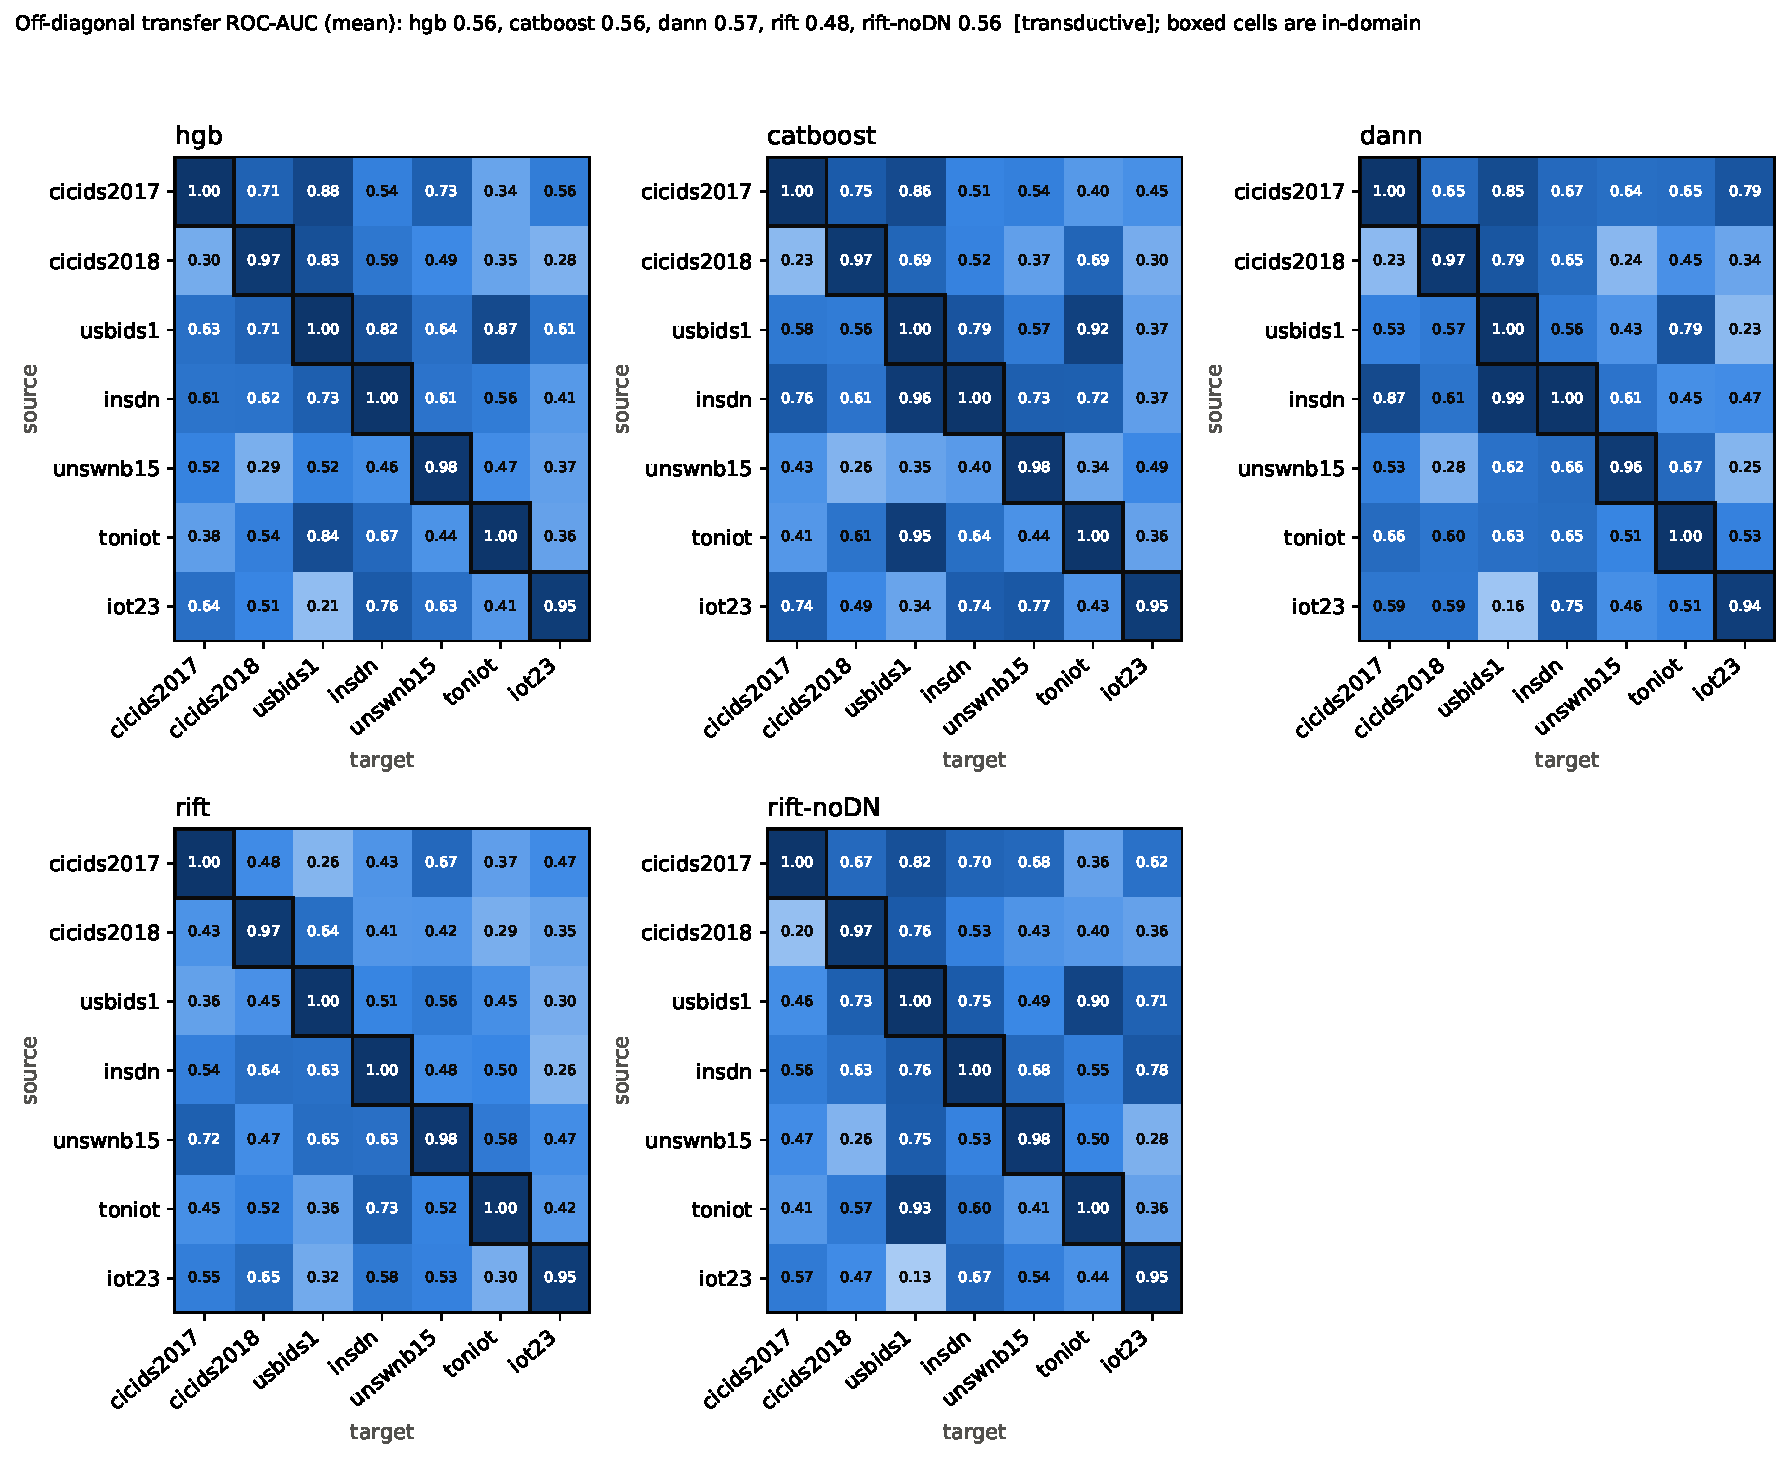
\includegraphics[width=0.9\textwidth]{figures/pairwise_matrix.pdf}
\caption{Source$\rightarrow$target ROC-AUC of the benchmark methods (transductive mode); the boxed diagonal is the in-domain value.}\label{fig:matrix}
\end{figure}

No method is consistently best.
A Friedman test over the 42 pairs finds a difference among the 17 transductive variants ($p=0.006$), but that is driven by the weak methods (logistic regression and the RIFT variants); among the inductive methods ($p=0.74$) and in LODO ($p=0.065$ transductive, $0.47$ inductive) it finds none.
The pairwise differences among CatBoost, HGB, XGBoost and DANN are of the order of 0.01 (in LODO up to 0.04, with CatBoost best on mean rank), far below the spread between pairs; with 7 LODO targets and pairs that share sources and targets, the Friedman tests have little power, so the data neither show nor exclude a best method.
On average CORAL and DANN do not repair transfer: pairwise they are at 0.524 and 0.565, in LODO at 0.631 and 0.613, against 0.630 for HGB, although both differ strongly by target (on LODO IoT-23 CORAL reaches 0.72 and DANN 0.76 against 0.31 for HGB).

\subsection{RIFT fails}
Table~\ref{tab:rift} shows RIFT and its ablations.
RIFT is below its own HGB baseline in both settings (pairwise 0.484 against 0.557, LODO 0.519 against 0.630).
Removing domain normalisation recovers the baseline (0.558 pairwise, 0.620 LODO), and removing the benign anchor recovers part of it (0.538, 0.543), so the target-side normalisation and the benign anchor are what hurt.
Removing the label-shift correction changes nothing (0.484 against 0.484 pairwise), as it must for ROC-AUC, because a prior-ratio adjustment is a monotone transform of the posterior.
In LODO the invariant selection has no effect either, for a mechanical reason: no feature has the same sign in all six sources (consistent with Sect.~\ref{sec:diag}), so the selection falls back to keeping all 13 features in every LODO scenario; in the pairwise setting the Kolmogorov--Smirnov rule keeps 10 of 13.
Replacing the rank transform by robust or z-score scaling does not help (0.479 and 0.485 pairwise).
Self-training does not help (0.478).
In the inductive pairwise setting there is no target pool and a single source, so RIFT keeps all features and reduces to HGB on a monotone rank transform; all variants score the same (0.551 against 0.554 for HGB).
In inductive LODO the per-domain source normalisation and the multi-source selection remain active and the variants differ (RIFT 0.586, without domain normalisation 0.620, robust scaling 0.502); RIFT is below HGB there too (0.630), and removing domain normalisation raises the score without any target data.

\begin{table}[t]
\centering\small
\caption{RIFT and its ablations, transductive mode. Pairwise: 42 pairs; LODO: 7 targets. Prior error (pairwise only): mean absolute error of the estimated target attack prior. Rows marked with an asterisk are oracle diagnostics that read the labels of the target pool.}\label{tab:rift}
\resizebox{\linewidth}{!}{\begin{tabular}{lrrrr}
\toprule
Method & Pairwise AUC & Pairwise bal. acc. & LODO AUC & Prior error \\
\midrule
HGB & 0.557 & 0.533 & 0.630 & -- \\
RIFT & 0.484 & 0.510 & 0.519 & 0.413 \\
RIFT $-$ domain norm. & 0.558 & 0.536 & 0.620 & 0.385 \\
RIFT $-$ benign anchor & 0.538 & 0.521 & 0.543 & 0.381 \\
RIFT $-$ invariant selection & 0.483 & 0.495 & 0.519 & 0.429 \\
RIFT $-$ prior correction & 0.484 & 0.509 & 0.519 & -- \\
RIFT, pooled init. & 0.487 & 0.500 & 0.498 & 0.421 \\
RIFT, robust scaling & 0.479 & 0.504 & 0.487 & 0.425 \\
RIFT, z-score scaling & 0.485 & 0.498 & 0.510 & 0.414 \\
RIFT + self-training & 0.478 & 0.507 & 0.500 & 0.409 \\
RIFT, true prior* & 0.488 & 0.503 & 0.562 & 0.000 \\
RIFT, true prior and anchor* & 0.543 & 0.507 & 0.596 & 0.000 \\
\bottomrule
\end{tabular}
}
\end{table}

The target-prior estimate is poor, although removing the correction does not matter for ROC-AUC and the prior error is similar for the variants that recover the baseline (0.39 and 0.38 for the variants without domain normalisation and without anchor against 0.41 for RIFT), so the error alone does not explain the loss.
Across the 42 pairs RIFT estimates the target attack prior with a mean absolute error of 0.41 (bias $-0.35$, Pearson correlation with the true prior 0.05); in LODO it estimates an average prior of 0.003 where the true average is 0.51.
The anchor is meant to be benign traffic, but its purity (the fraction of truly benign rows, logged as a diagnostic and never used by the method) is 0.50 in pairwise and 0.47 in LODO transfer, so the anchor is as contaminated with attacks as the pool.
Estimating the prior with a normaliser fitted on the pool (``pooled init.'') does not help (0.487).
We hypothesise, without having tested it, that a source classifier that is inverted on the target gives the EM nothing to correct.

\paragraph{Oracle diagnostics.}
Two diagnostics read the labels of the target pool and are therefore not label-free methods.
Supplying the true target prior to the anchor and to the correction gives 0.488 pairwise and 0.562 LODO, and the anchor stays as contaminated (purity 0.48 and 0.49), so a perfect prior estimate does not repair RIFT.
Additionally replacing the anchor by truly benign pool rows gives 0.543 and 0.596, which recovers most of RIFT's loss but stays below HGB (0.557 and 0.630), and balanced accuracy stays at 0.51.
The benign anchor therefore matters, but with perfect information the target-side normalisation still does not improve on no adaptation, which is consistent with the failure lying in the rule that the source classifier carries and not in the estimation of the shift.

\begin{figure}[t]
\centering
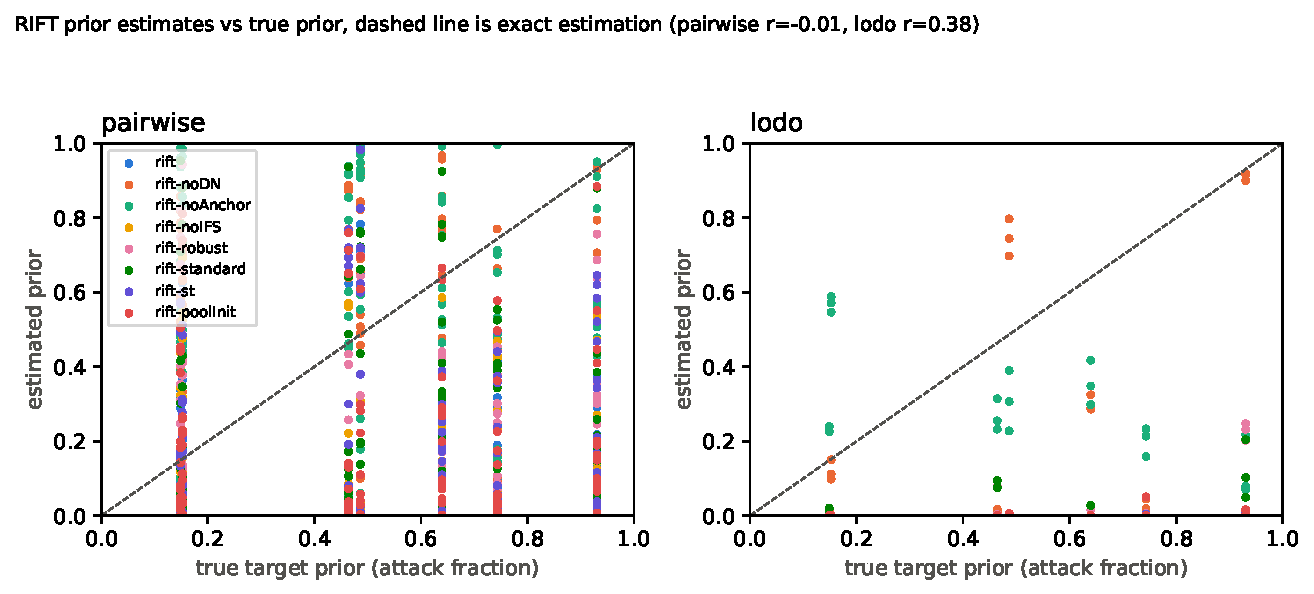
\includegraphics[width=0.75\textwidth]{figures/prior_estimation.pdf}
\caption{Estimated against true target attack prior for the RIFT variants.}\label{fig:prior}
\end{figure}

\subsection{Source data do not help in the few-label setting}
As a reference outside the label-free benchmark, we continue a source-pretrained CatBoost on a labelled budget of 0.1\%, 1\% and 5\% of the target training split (on average 62, 617 and 3\,083 rows), and compare it with CatBoost trained on those rows alone.
At 0.1\%, the source-pretrained model reaches 0.835 and the target-only model 0.928 (Table~\ref{tab:fewshot}).
Giving the continued model 300 or 500 extra trees narrows the gap to 0.911 and 0.914 against 0.932, so the effect is not only a capacity artefact, but it does not reverse: at 1\% and 5\% the two are within 0.001 to 0.002 once the trees are matched.
Source pre-training thus gives no average benefit over target labels for this model family, and a harm at the smallest budget (0.09 AUC with 100 trees, 0.02 with 500); continuing a boosted model by adding trees is a weak way to use source data, and stronger few-label baselines (pooled training with target weighting, source scores as a feature, an in-context model given the source rows) are not part of this study.

\begin{table}[t]
\centering\small
\caption{Few-label comparison over the 42 pairs, ROC-AUC. The continued model starts from a CatBoost trained on the source and adds the stated number of trees on the labelled target rows; the other model uses only those rows.}\label{tab:fewshot}
\begin{tabular}{lrrrr}
\toprule
Setting & Extra trees & 0.1\% labels & 1\% labels & 5\% labels \\
\midrule
Source-pretrained, continued & 100 & 0.835 & 0.950 & 0.966 \\
 & 300 & 0.911 & 0.966 & 0.978 \\
 & 500 & 0.914 & 0.966 & 0.978 \\
Target labels only & 100 & 0.928 & 0.964 & 0.977 \\
 & 300 & 0.932 & 0.967 & 0.980 \\
 & 500 & 0.932 & 0.967 & 0.979 \\
\bottomrule
\end{tabular}

\end{table}

\subsection{Shift and family explanations}
An unsupervised shift score (an isolation forest fitted on the source and applied to the target pool) does not predict transfer skill: the Spearman correlation with zero-shot ROC-AUC over 2\,142 (scenario, method, seed) points is $-0.055$ (nominal $p=0.01$, but the points are not independent; per method $|\rho|\le0.27$ with mixed signs).
Sharing attack types does not obviously predict it either: for every family we compared the informedness of a method on a target family when the source contains that family and when it does not.
Pooled over families (transductive mode), the paired difference for CatBoost is $+0.012$ (95\% half-width 0.088, $p=0.82$) and for HGB $-0.046$ ($p=0.14$); none of the 248 (method, mode, family) tests has $p<0.05$, but each test uses only 3 to 6 paired cells and cannot reach 0.05 with fewer than 6, so the benchmark has too little power to show whether missing attack types matter.

\subsection{Controls on the diagnosis}\label{sec:diag}
A negative result is a finding only if competing explanations are ruled out.
\paragraph{The pipeline works.}
The same pipeline reaches 0.985 in-domain, and a target-only CatBoost with 0.1\% of target labels reaches 0.93, so the features carry the signal and the code can learn it.

\paragraph{Tuning as an explanation (one informative pair).}
For CIC-IDS2017$\rightarrow$CIC-IDS2018 we searched all five model families (HGB, CatBoost, XGBoost, random forest, logistic regression) with two settings of the main hyperparameters, three normalisations (none, global, per-domain rank) and the full feature set or the set without one feature group (264 configurations, seed 0, 30\,000 source rows), and selected the best on the target test split, an optimistic oracle.
It reaches 0.799 against 0.683 for the benchmark HGB, still far from the in-domain 0.97 to 1.00.
For CIC-IDS2017$\rightarrow$USB-IDS-1 only 33 HGB configurations were run and the oracle (0.862) is below the full-data benchmark HGB (0.972), so that pair says nothing about tuning.
The grid is reduced and the source is subsampled, so the result is not an upper bound over all configurations.

\paragraph{The same statistics do not carry the same labels.}
We standardise source and target with source statistics, find for each target row its 10 nearest source rows, and restrict to the \emph{overlap region} (rows whose mean neighbour distance is at most the 90th percentile of source-to-source distances).
There the majority label of the neighbours should agree with the true target label if $P(y\mid x)$ were shared.
Over the 19 pairs with at least 100 overlapping rows (seed 0; 23 of the 42 pairs have fewer) the median Cohen's $\kappa$ is 0.03, 84\% of the pairs have $\kappa\le0.1$ and the maximum is 0.25 (Fig.~\ref{fig:kappa}); three of the 19 values are exactly 0, which a single-class overlap region also produces, and only five are negative, so the pattern is closer to independence than to inversion. The in-domain reference, source-test rows against the same source-train index, has $\kappa$ of 0.91 on average and is not matched in region or difficulty.
The pair CIC-IDS2017$\rightarrow$CIC-IDS2018, from one laboratory, has $\kappa=-0.07$ with 40\% of the target rows in the overlap region.

\begin{figure}[t]
\centering
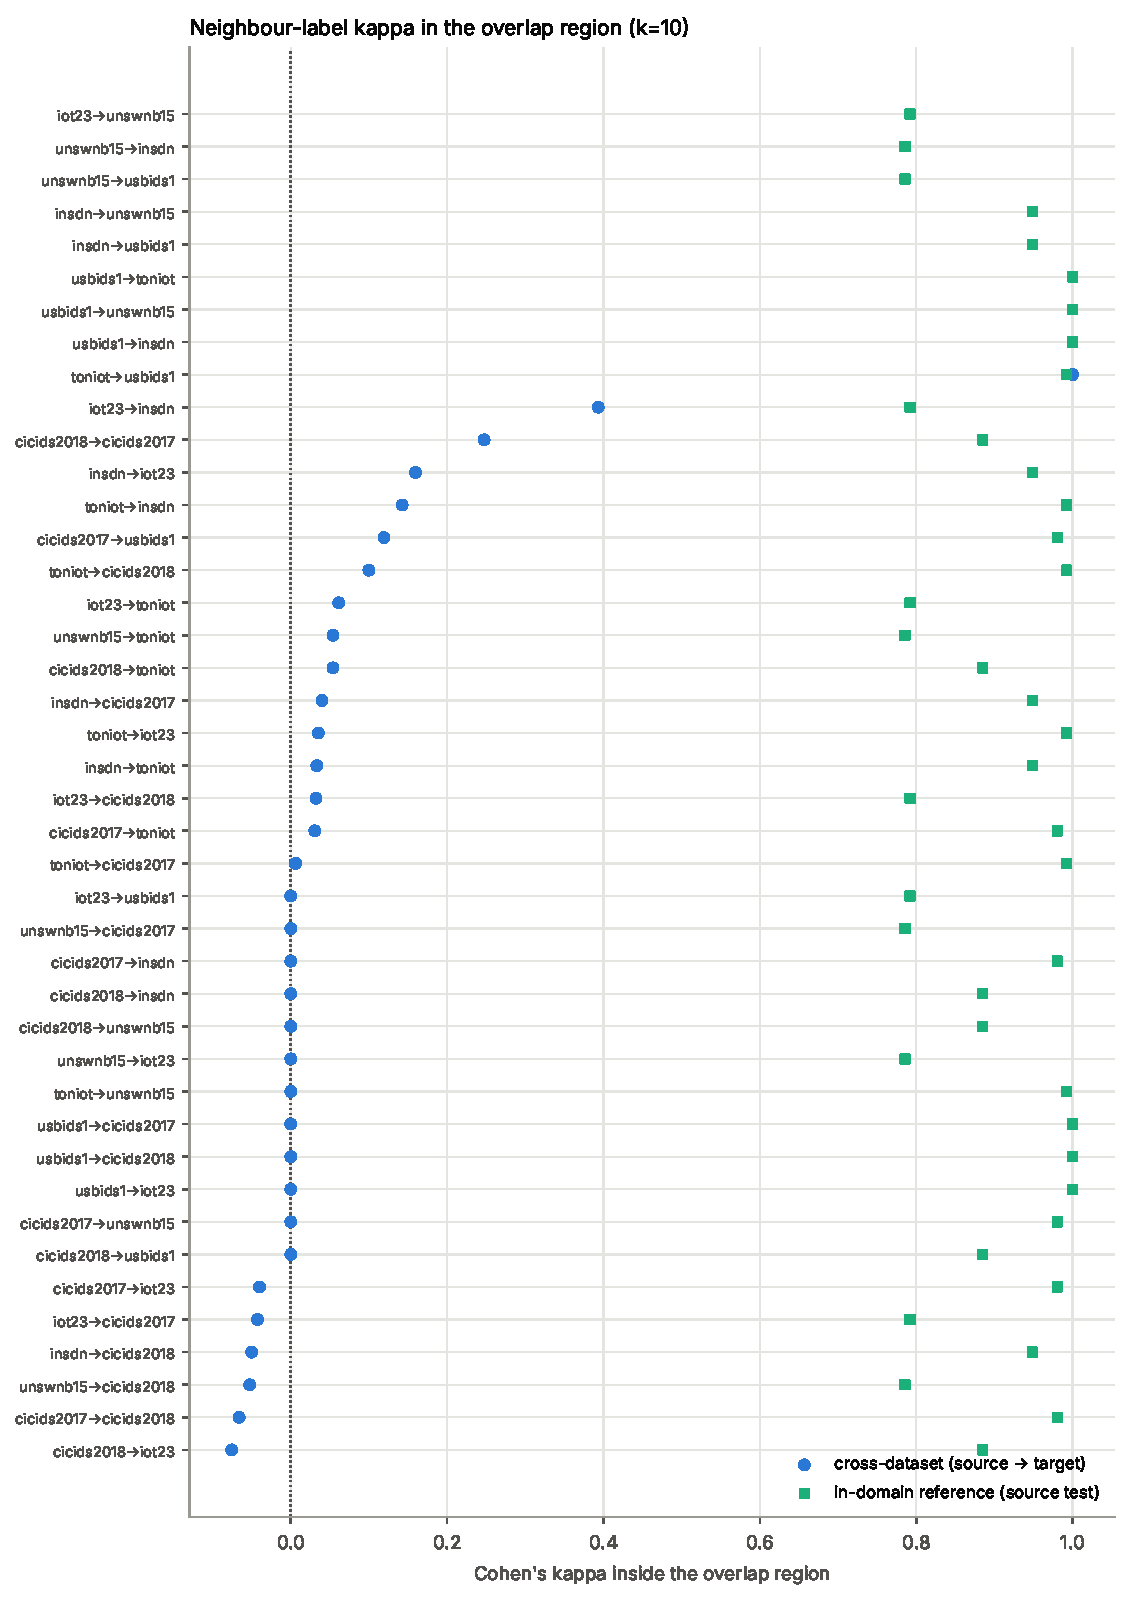
\includegraphics[width=0.8\textwidth]{figures/concept_kappa.pdf}
\caption{Cohen's $\kappa$ between the majority label of the nearest source rows and the true target label in the overlap region, per pair, against the in-domain reference.}\label{fig:kappa}
\end{figure}

\paragraph{The same attack family does not transfer either.}
For every attack family present in at least two core datasets with at least 200 rows each (DoS, DDoS, scan, brute force, exploit/malware and botnet; families assigned by name rules in \texttt{crossids.analysis}) we trained HGB on benign flows plus that family in one dataset and scored benign flows plus that family in another: 74 ordered dataset--family cells with up to 20\,000 rows per class (Table~\ref{tab:family}).
The median cross-dataset ROC-AUC is 0.545, 36\% of the cells are below 0.5, 7\% reach 0.8 and none reaches 0.9, whereas the in-domain version of the same task has median 1.000 (minimum 0.82).
The attack mix is thus held fixed up to the coarse family and transfer still fails, which excludes a difference of attack mix alone.
It does not separate a change of the conditional label distribution from differences in benign traffic and in how flows are measured, since benign flows also differ between datasets (below); the family assignment is coarse (DoS covers different tools), and the botnet family has two cells.

\begin{table}[t]
\centering\small
\caption{Transfer of a single attack family between datasets: HGB trained on benign plus the family in the source dataset, ROC-AUC on benign plus the family in the target dataset (seed 0, up to 20\,000 rows per class).}\label{tab:family}
\begin{tabular}{lrrrrr}
\toprule
Family & Cells & Median cross-dataset AUC & Min & Max & Median in-domain AUC \\
\midrule
DoS & 30 & 0.569 & 0.313 & 0.857 & 0.999 \\
DDoS & 12 & 0.526 & 0.245 & 0.750 & 1.000 \\
Scan & 12 & 0.598 & 0.120 & 0.900 & 1.000 \\
Brute force & 12 & 0.514 & 0.148 & 0.829 & 0.999 \\
Exploit / malware & 6 & 0.543 & 0.464 & 0.814 & 0.993 \\
Botnet & 2 & 0.366 & 0.042 & 0.689 & 0.918 \\
\midrule
All & 74 & 0.545 & 0.042 & 0.900 & 1.000 \\
\bottomrule
\end{tabular}

\end{table}

\paragraph{No flow feature keeps its meaning.}
For each feature we computed the univariate ROC-AUC with the label in every dataset.
The sign of the association (above or below 0.5) is mixed for all 14 features of the eight datasets (13 core features and the minimal-tier \texttt{bytes\_per\_pkt}) and also for all 13 core features of the seven core datasets, with per-dataset AUC ranges such as 0.025 to 0.760 for total bytes and 0.057 to 0.808 for forward packets (Fig.~\ref{fig:sign}).

\begin{figure}[t]
\centering
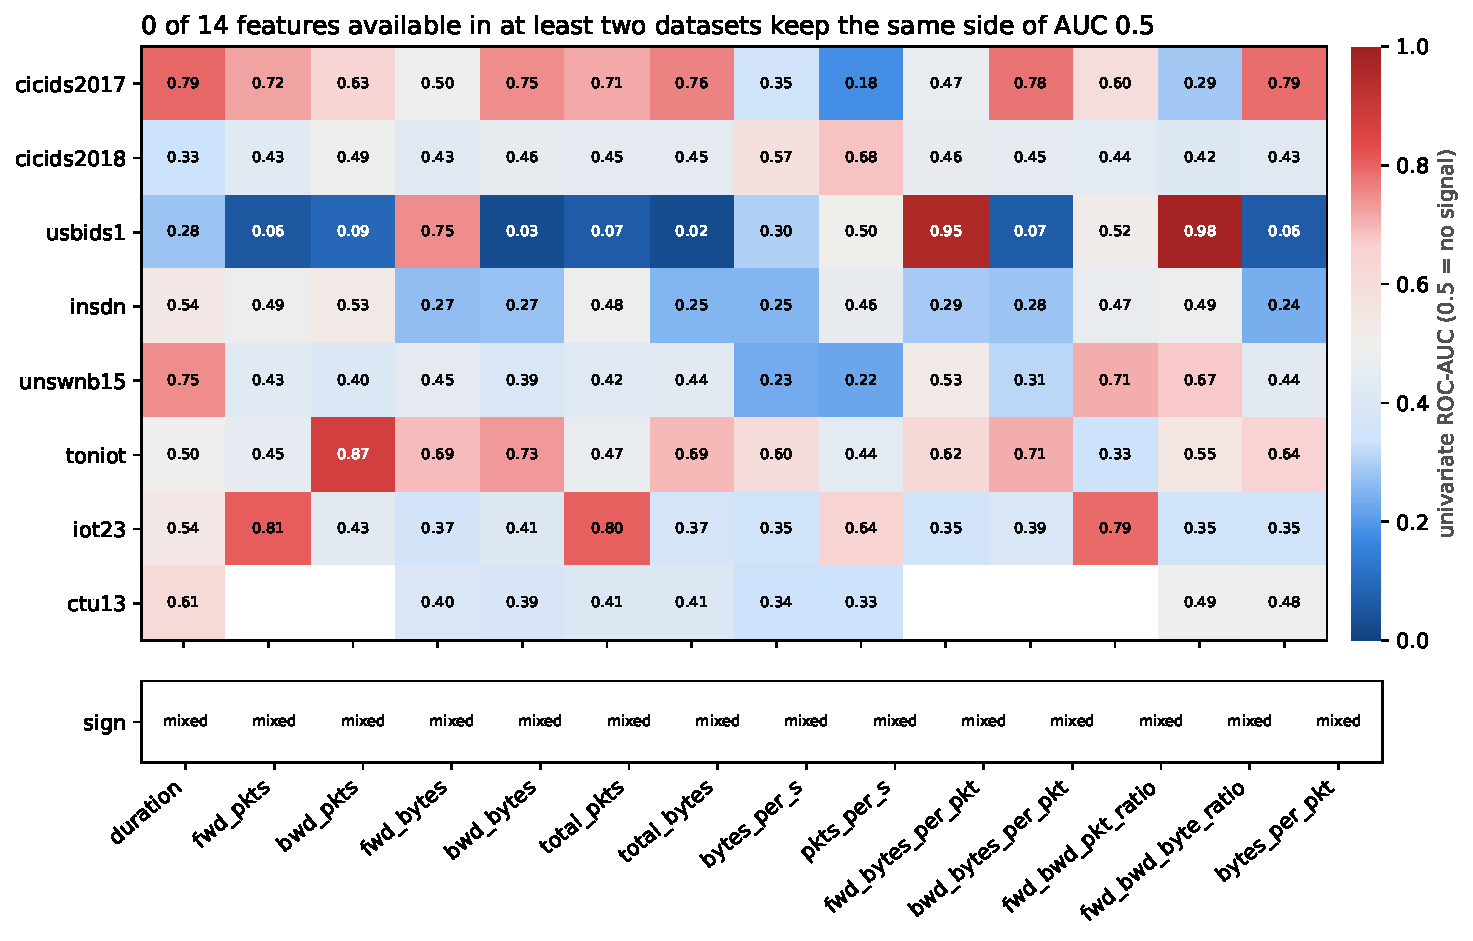
\includegraphics[width=0.9\textwidth]{figures/feature_sign.pdf}
\caption{Univariate ROC-AUC of each core feature with the attack label, per dataset (centred at 0.5); the figure includes CTU-13 and the minimal-tier feature \texttt{bytes\_per\_pkt}.}\label{fig:sign}
\end{figure}

\paragraph{Datasets are easy to tell apart.}
A CatBoost classifier recognises the dataset of a flow among the seven core datasets with 91.5\% accuracy (chance 14.3\%), and 91.8\% on benign flows alone.
Benign traffic therefore also differs between datasets, which is consistent with differences in capture setup and background traffic.

\paragraph{Published results agree.}
The reported collapses in the literature occur in the same regime: attack-class F1 below 1\% for several NetFlow-v2 pairs \citep{layeghy2023explainable}, MCC between 0.26 and 0.44 for CIC-IDS2017 and CIC-IDS2018 \citep{cantone2024crossdataset}.
Metrics and feature sets differ across studies, so we compare the pattern and not the numbers.

\begin{table}[t]
\centering\small
\caption{What each control can and cannot show.}\label{tab:controls}
\begin{tabular}{p{0.24\textwidth}p{0.34\textwidth}p{0.34\textwidth}}
\toprule
Control & Rules out & Cannot rule out \\
\midrule
In-domain skill (0.985) & A broken pipeline or uninformative features & Anything about transfer; in-domain tasks may be easy for testbed-generated attacks \\
Oracle search (one informative pair) & Default hyperparameters of HGB on that pair & Tuning in general (one pair, reduced grid, subsampled source) \\
Single-family transfer & A difference of attack mix alone & Differences in benign traffic, in measurement, and in the conditional label distribution \\
Nearest-neighbour $\kappa$ & Nothing alone: the overlap is small and $\kappa=0$ also arises from a single-class region & Shift in $P(y\mid x)$; the test has little power \\
Per-feature signs & A stable direction of any single feature & Attack-mix shift (no within-dataset null) \\
Dataset identity (91.5\%) & Datasets being interchangeable & Which kind of shift it is; it indicates large covariate or support shift \\
RIFT oracle diagnostics & Prior estimation as the cause of RIFT's failure & Other adaptation designs \\
Few-label comparison & Source pre-training by continuing boosted trees as useful on average & Better ways to use source data \\
\bottomrule
\end{tabular}
\end{table}

\section{Few-label transfer: FLARE-2 and a tabular foundation model}\label{sec:fewlabel}
The diagnosis of Sect.~\ref{sec:results} leaves a practical question: when a handful of target flows are labelled, what can the other datasets still contribute?
We study it as leave-one-dataset-out few-label transfer on eight targets (the seven benchmark datasets and CTU-13), with the target never seen in meta-training or checkpoint selection.
We first describe the setting and the baselines, then FLARE-2, and then the results.
In this setting a model receives a \emph{support set} of $k$ labelled target flows and must classify the other target flows (the \emph{query set}).
FLARE-2 is \emph{meta-trained}: it is trained on many small classification tasks (episodes) built from the other datasets, each with a support set and a query set, so that at test time it reads the labelled flows as input and classifies new ones without any gradient update on the target, which is called in-context learning.
TabPFN follows the same idea but is pretrained on synthetic tasks instead of network data.

\subsection{Setting}
We use leave-one-dataset-out (LODO): the target dataset is never seen in meta-training or checkpoint selection.
At test time a method receives a support set of $k\in\{4,8,16,32,64,128\}$ labelled target flows with at least one flow per class, and may use no other target label. FLARE-2 additionally ranks features over the unlabelled target rows it scores (Sect.~\ref{sec:method}); the baselines receive no such information.
Support sets are drawn 10 times per $(\text{target},k)$ with fixed seeds and are identical for every method.
Evaluation is on the target test split.
For class level we use $k\in\{2,4,8,16\}$ labelled flows \emph{per class} and 5 draws (InSDN only up to $k=8$ per class, because its attack classes are small).


Table~\ref{tab:zero} shows the zero-shot picture: a CatBoost trained on all other datasets (LODO) scores from 0.322 (IoT-23) to 0.952 (USB-IDS-1), below chance on three targets (IoT-23, CTU-13, UNSW-NB15).

\begin{table}[t]
\centering\small
\caption{Zero-shot ROC-AUC on the target test split ($k=0$). LODO: CatBoost on all other datasets pooled. Pairwise: mean and best single source from the pairwise benchmark (not computed for CTU-13). Full label: CatBoost trained on the full target train split.}\label{tab:zero}
\begin{tabular}{lcccc}
\toprule
Target & CatBoost LODO & pairwise mean & pairwise best & full label \\
\midrule
CIC-IDS2017 & 0.832 & 0.559 & 0.761 & 0.999 \\
CIC-IDS2018 & 0.656 & 0.547 & 0.698 & 0.968 \\
CTU-13 & 0.358 & -- & -- & 0.962 \\
InSDN & 0.730 & 0.598 & 0.827 & 0.998 \\
IoT-23 & 0.322 & 0.370 & 0.460 & 0.950 \\
ToN-IoT & 0.608 & 0.593 & 0.942 & 0.999 \\
UNSW-NB15 & 0.485 & 0.585 & 0.781 & 0.977 \\
USB-IDS-1 & 0.952 & 0.695 & 0.965 & 1.000 \\
\bottomrule
\end{tabular}

\end{table}

\subsection{Baselines, tabular foundation models and statistics}
\paragraph{Baselines on identical supports.}
Random forest (RF), CatBoost \citep{prokhorenkova2018catboost}, logistic regression (LR) and $k$NN trained on the $k$ target labels only; CatBoost pretrained on the sources and fine-tuned on the $k$ labels (the earlier approach); and, as zero-shot references, CatBoost trained on all other datasets and the pairwise single-source results.
Baselines use fixed standard settings and no tuning (RF: 300 trees; CatBoost: 300 iterations, depth 6, learning rate 0.05; LR and $k$NN with up to 5 neighbours on standardised features; class-balanced weights), since selecting hyperparameters from a handful of labels is itself unreliable; a baseline tuned with extra target labels could be stronger.
For $N$-way, baselines are the multi-class versions trained on the labelled $k$ per class.
\paragraph{Tabular foundation models.}
TabPFN \citep[the family of][]{hollmann2025tabpfn}, versions 3 and 3.5 (released weights of the \texttt{tabpfn} package, version 9.2.0, and of the \texttt{Prior-Labs/tabpfn\_3} repository), with default settings and the same support and query rows as every other method.
We did not train or tune the models on network data (the model card of version 3 states that it is trained purely on synthetic tabular tasks \citep{priorlabs2026tabpfn3}; we have not verified the pretraining data of version 3.5); they read the support set as training data and score each query row independently of the other query rows, so, unlike FLARE-2, they do not use the unlabelled target rows.
Version 3.5 was run for all three meta-training seeds and version 3 for seed 0.
At class level TabPFN-3.5 was run for seed 0 with five draws (the draws of FLARE-2): on all query rows of IoT-23, ToN-IoT and CTU-13, and, to save time, on a fixed stratified subsample of at most 5\,000 query rows per task for the other five targets; scoring IoT-23 both ways changes the class-level metrics by at most 0.005 on average (per-class ROC-AUC $+0.002$, macro-F1 $+0.001$, recall $+0.005$).
The weights are released under a non-commercial research license, which applies here.
\paragraph{Metrics and statistics.}
ROC-AUC (binary and per class), recall and false-positive rate at threshold 0.5, and macro-F1 for $N$-way classification.
Draws of one target are not independent, so the unit of analysis is the \emph{target}: the mean difference of FLARE-2 minus baseline over draws, then an exact two-sided Wilcoxon signed-rank test over the 8 targets (smallest attainable $p=0.0078$), Holm-adjusted over the five baselines (four at class level in the three-seed analysis; Table~\ref{tab:class} reports uncorrected seed-0 $p$), and a 95\% bootstrap interval over targets. Only the mean over $k$ is a primary endpoint; the $k\le16$ and $k\ge32$ splits are exploratory.
For class-level results we also report units of (target, class), with a warning that classes of one target are correlated; the target-level test is the conservative one.

\subsection{FLARE-2}\label{sec:method}
FLARE-2 classifies a query flow by attending to labelled support flows of the same episode.
At test time the episode is the $k$ support flows and the query flows; nothing is trained.

\paragraph{Episode normalisation.}
Within an episode, each feature is mapped to its Gaussian rank over support and query rows and clipped to $[-4,4]$. At test time the query rows are the whole unlabelled target test split (and, for per-class evaluation, only the rows of the class and of benign), whereas training episodes rank over 256 query rows, so FLARE-2 is transductive in the target features and the per-class pool depends on the class labels of the test rows. A control with a reference of 256 query rows, as in training, gives the same ROC-AUC (Sect.~\ref{sec:fewcontrols}).
Absolute scales, which differ across extractors, therefore never reach the network.
Missing features are absent tokens.

\paragraph{Tokens and layers.}
Flow $i$ with features $x_{i1},\dots,x_{id}$ becomes $d$ feature tokens $t_{ij}=\mathrm{MLP}_v(x_{ij})$ with a shared scalar embedding, plus one label token.
There is no feature-identity embedding, so the model cannot memorise that ``feature 7 high means attack'' and is invariant to feature order.
Six layers of width 128 with 4 heads alternate \emph{feature attention} (tokens of one row attend to each other) and \emph{row attention} (rows attend across the episode).
Support rows attend to support rows; a query row attends to support rows and itself only, so attention does not depend on which other queries share the batch; the rank normalisation above does.

\paragraph{Label slots and matching readout.}
Class identities differ between episodes, so each support class is given a random one of $M=16$ label-slot embeddings as input.
The readout does not index slots.
Each row is summarised by the layer-normalised mean $r_i$ of its tokens; a query gives $q=W_q r$, a support row $s$ gives key $k_s=W_k r_s$, and the logit of an active class $j$ with support $S_j$ is
\begin{equation}
\ell_j=\log\!\!\sum_{s\in S_j}\exp\!\Big(\frac{\langle q,k_s\rangle}{\sqrt{w}\,\tau}\Big)-b\log|S_j|,
\end{equation}
with $w=128$, a learned temperature $\tau>0$ and a learned $b\in[0,1]$ that interpolates between sum and mean pooling over a class's keys.
A softmax over the $N$ active classes is trained with cross-entropy.
The head is equivariant to permutations of classes and slots by construction and serves binary detection ($N=2$) and attack-type classification alike.
A slot-indexed linear head plateaued in training and was replaced by this one.
At test time we average class logits over 8 members with different sign flips and class-to-slot maps.

\paragraph{Meta-training episodes.}
Each episode draws a source dataset (weighted by $\sqrt{\text{size}}$) and a \emph{task}: binary attack vs benign (probability 0.25), one attack class vs benign (0.25), class vs class (0.15), or $N$-way with $N\sim U\{3..6\}$ among benign and attack classes (0.35).
Raw attack types with fewer than 30 rows are dropped.
The per-class support size is log-uniform on $\{1,\dots,32\}$ with at most 160 support rows in total, so a binary episode never has more than 64 support rows while evaluation uses up to 128; the query class proportions are Dirichlet(1) with at least one query row per class, so no fixed prior can be learned; 30\% of binary, one-class and $N$-way episodes (about 25\% of all episodes) combine benign rows of one dataset with attack classes of another; with probability 0.5 a random subset of at least 5 features is kept; 2\% of support labels are flipped; each feature is sign-flipped independently with probability 0.5.
A monotone warp was also tried; it has no effect under rank normalisation and was dropped.
Because both the meaning of a class and the sign of every feature change from episode to episode, the only reliable strategy is to read the rule from the support set.
This is the design response to the concept shift of Sect.~\ref{sec:diag}; Sect.~\ref{sec:ablation} measures how much the individual choices, including the class-level tasks, contribute, and the evidence for them is modest.

\paragraph{Held-out-source model selection.}
Our first variant added unlabelled context rows from the target network.
It reached 0.97 AUC on validation episodes from the meta-training datasets but fell to 0.66--0.76 on the unseen IoT-23 target: with datasets identifiable at 91\%, six binary tasks are easy to memorise.
In FLARE-2, one source dataset (rotating, never the target) is excluded from training and used only to select the checkpoint with the lowest validation loss.
The unlabelled-context variant is not part of FLARE-2.

\paragraph{Training.}
AdamW (learning rate $3\times10^{-4}$, weight decay 0.01, cosine schedule, 1k warm-up steps), 20k steps, 8 episodes per step, 256 query rows, gradient clipping at 1.0, mixed-precision autocast (fp16 on a Colab T4 for the main runs, bf16 on a local RTX GPU for the ablation runs and extra seeds).
One model is trained per target (LODO), about 1 hour each.
The label-slot readout computes in float32 to avoid half-precision overflow.

\subsection{Binary detection}
Table~\ref{tab:binary} and Fig.~\ref{fig:curves} show ROC-AUC versus $k$.
With $k=4$ labelled flows, FLARE-2 already beats the zero-shot pooled CatBoost on five of eight targets (CTU-13, IoT-23, ToN-IoT, UNSW-NB15, USB-IDS-1; Tables~\ref{tab:zero},~\ref{tab:binary}); on the other three (CIC-IDS2017, CIC-IDS2018, InSDN), where pooled sources transfer well, 8 to 16 labelled flows are needed to catch up.
Table~\ref{tab:stats} gives the paired statistics.
Against the strongest baselines the difference is small and not significant: mean over $k$, FLARE-2 minus target-only CatBoost is $-0.001$ and minus RF is $+0.004$; both intervals contain zero and the win/loss counts over targets are 4/4 and 5/3.
Against LR and $k$NN the gain is large: FLARE-2 is higher on all 8 targets for the mean over $k$ ($+0.075$ and $+0.110$, $p_{\text{Holm}}=0.039$ for both).
Against source-pretrained CatBoost fine-tuned on the labels, seed 0 shows FLARE-2 better for $k\ge 32$ (7 of 8 targets, $p_{\text{Holm}}=0.047$) and not different below; the repeat over seeds below shows that this advantage is not robust.

\paragraph{Three meta-training seeds.}
We repeated the benchmark (meta-training, the split of the target and the support draws) with seeds 1 and 2 on all eight targets, for FLARE-2 and every baseline.
Table~\ref{tab:seeds} gives the paired differences with the target as unit, after averaging each target over the three seeds.
The seed-averaged differences to RF and to target-only CatBoost are $+0.001$ and $-0.001$ for the mean over $k$ (per seed $-0.002$ to $+0.004$), and the standard deviation over seeds of the mean difference is 0.001 to 0.009 across the rows of Table~\ref{tab:seeds}, so training variance is small next to the spread between targets.
FLARE-2 stays above LR and $k$NN on all 8 targets in every scope ($p_{\text{Holm}}=0.039$).
The seed-0 advantage over fine-tuned CatBoost at $k\ge 32$ shrinks to $+0.007$ (5 of 8 targets, $p_{\text{Holm}}=0.33$), and the mean difference over $k$ is $+0.002$ (CI $[-0.015,+0.020]$).
We therefore claim neither superiority nor inferiority to the tree ensembles on binary ROC-AUC.

\begin{table}[t]
\centering\small
\caption{FLARE-2 minus baseline in binary ROC-AUC, mean over meta-training seeds 0--2, unit = target (8). W/L: targets where FLARE-2 is higher / lower. SD: standard deviation over seeds of the mean difference. $p_{\text{Holm}}$: exact Wilcoxon over targets, Holm-adjusted over the five baselines within each scope. Only the mean over $k$ is a primary endpoint.}\label{tab:seeds}
\resizebox{\linewidth}{!}{\begin{tabular}{llrrrrr}
\toprule
Scope & Baseline & Mean diff. & 95\% CI & W/L & SD over seeds & $p_{\text{Holm}}$ \\
\midrule
mean over k & RF & +0.001 & [-0.004, +0.006] & 4/4 & 0.003 & 1.000 \\
 & CatBoost (target only) & -0.001 & [-0.004, +0.002] & 4/4 & 0.001 & 1.000 \\
 & CatBoost (source + fine-tune) & +0.002 & [-0.015, +0.020] & 3/5 & 0.004 & 1.000 \\
 & LR & +0.073 & [+0.044, +0.102] & 8/0 & 0.003 & 0.039 \\
 & kNN & +0.113 & [+0.090, +0.135] & 8/0 & 0.004 & 0.039 \\
\midrule
k$\leq$16 & RF & +0.002 & [-0.006, +0.012] & 3/5 & 0.003 & 1.000 \\
 & CatBoost (target only) & -0.002 & [-0.008, +0.004] & 3/5 & 0.001 & 1.000 \\
 & CatBoost (source + fine-tune) & -0.004 & [-0.034, +0.030] & 3/5 & 0.003 & 1.000 \\
 & LR & +0.082 & [+0.046, +0.118] & 8/0 & 0.005 & 0.039 \\
 & kNN & +0.174 & [+0.131, +0.215] & 8/0 & 0.009 & 0.039 \\
\midrule
k$\geq$32 & RF & -0.001 & [-0.004, +0.004] & 2/6 & 0.003 & 1.000 \\
 & CatBoost (target only) & -0.000 & [-0.003, +0.002] & 3/5 & 0.003 & 1.000 \\
 & CatBoost (source + fine-tune) & +0.007 & [+0.002, +0.012] & 5/3 & 0.005 & 0.328 \\
 & LR & +0.064 & [+0.035, +0.095] & 8/0 & 0.005 & 0.039 \\
 & kNN & +0.051 & [+0.037, +0.066] & 8/0 & 0.005 & 0.039 \\
\bottomrule
\end{tabular}
}
\end{table}

\begin{table}[t]
\centering\scriptsize
\caption{Binary ROC-AUC, mean over 10 support draws. F2: FLARE-2; RF: random forest; CB: CatBoost on target labels; CB-ft: source-pretrained CatBoost fine-tuned on the labels. TP3.5: TabPFN-3.5. Bold marks the best of the five.}\label{tab:binary}
\resizebox{\textwidth}{!}{\begin{tabular}{lccccccccccccccc}
\toprule
& \multicolumn{5}{c}{$k=4$} & \multicolumn{5}{c}{$k=16$} & \multicolumn{5}{c}{$k=64$} \\
\cmidrule(lr){2-6}\cmidrule(lr){7-11}\cmidrule(lr){12-16}
Target & F2 & RF & CB & CB-ft & TP3.5 & F2 & RF & CB & CB-ft & TP3.5 & F2 & RF & CB & CB-ft & TP3.5 \\
\midrule
CIC-IDS2017 & 0.785 & 0.718 & 0.754 & \textbf{0.841} & 0.747 & 0.861 & \textbf{0.888} & 0.861 & 0.880 & 0.887 & 0.965 & 0.966 & 0.969 & 0.956 & \textbf{0.979} \\
CIC-IDS2018 & 0.605 & 0.599 & 0.604 & \textbf{0.691} & 0.611 & 0.695 & 0.657 & 0.711 & \textbf{0.733} & 0.713 & 0.892 & 0.884 & 0.880 & 0.875 & \textbf{0.904} \\
CTU-13 & 0.599 & 0.599 & 0.599 & 0.470 & \textbf{0.633} & 0.704 & 0.700 & \textbf{0.718} & 0.648 & 0.709 & 0.797 & 0.806 & 0.797 & 0.783 & \textbf{0.807} \\
InSDN & 0.644 & 0.671 & 0.690 & \textbf{0.804} & 0.659 & 0.901 & 0.872 & 0.875 & 0.890 & \textbf{0.911} & 0.960 & 0.956 & 0.954 & 0.949 & \textbf{0.970} \\
IoT-23 & 0.785 & 0.825 & \textbf{0.839} & 0.763 & 0.819 & 0.877 & 0.876 & 0.852 & 0.857 & \textbf{0.886} & 0.905 & 0.894 & 0.900 & 0.891 & \textbf{0.911} \\
ToN-IoT & 0.720 & 0.716 & 0.723 & 0.679 & \textbf{0.767} & 0.899 & 0.861 & 0.885 & 0.893 & \textbf{0.910} & 0.961 & 0.968 & 0.968 & 0.960 & \textbf{0.975} \\
UNSW-NB15 & 0.647 & 0.679 & 0.682 & 0.625 & \textbf{0.685} & 0.794 & 0.809 & 0.788 & 0.767 & \textbf{0.821} & 0.870 & 0.875 & 0.871 & 0.859 & \textbf{0.882} \\
USB-IDS-1 & 0.978 & 0.958 & 0.972 & \textbf{0.983} & 0.969 & 0.957 & 0.993 & \textbf{0.997} & 0.994 & 0.994 & 0.997 & 0.999 & 0.999 & 0.998 & \textbf{1.000} \\
\bottomrule
\end{tabular}
}
\end{table}

\begin{figure}[t]
\centering
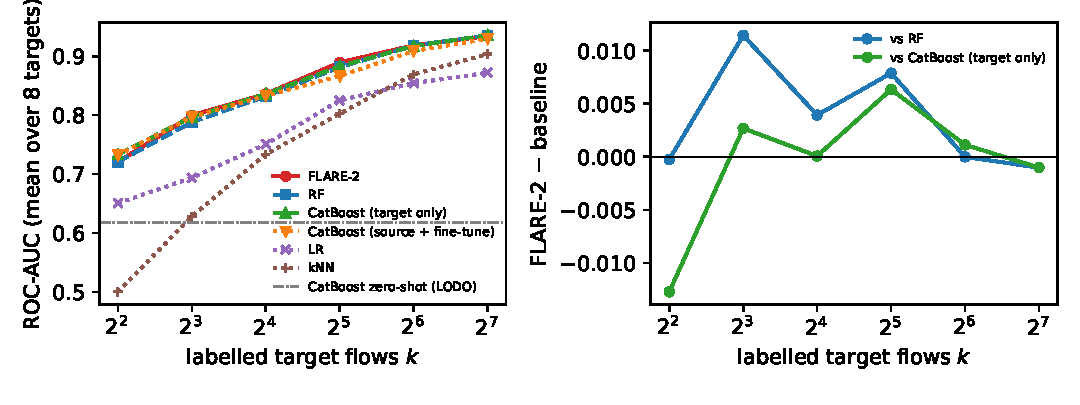
\includegraphics[width=\textwidth]{figures/curves.pdf}
\caption{Left: ROC-AUC against $k$, mean over the eight targets. Right: FLARE-2 minus RF and minus target-only CatBoost.}\label{fig:curves}
\end{figure}

\begin{table}[t]
\centering\small
\caption{Paired differences in binary ROC-AUC (FLARE-2 minus baseline), unit = target (8). W/L: targets where FLARE-2 is higher / lower. $p_{\text{Holm}}$: exact Wilcoxon over targets, Holm-adjusted over baselines.}\label{tab:stats}
\begin{tabular}{llcccc}
\toprule
Scope & Baseline & $\Delta$ROC-AUC & 95\% CI & W/L & $p_{\text{Holm}}$ \\
\midrule
mean over k & RF & +0.004 & [-0.003, +0.010] & 5/3 & 1.000 \\
mean over k & CatBoost (target) & -0.001 & [-0.004, +0.003] & 4/4 & 1.000 \\
mean over k & CatBoost (fine-tune) & +0.005 & [-0.010, +0.022] & 4/4 & 1.000 \\
mean over k & LR & +0.075 & [+0.044, +0.106] & 8/0 & 0.039 \\
mean over k & kNN & +0.110 & [+0.085, +0.133] & 8/0 & 0.039 \\
k$\leq$16 & RF & +0.005 & [-0.004, +0.014] & 4/4 & 1.000 \\
k$\leq$16 & CatBoost (target) & -0.003 & [-0.009, +0.002] & 4/4 & 1.000 \\
k$\leq$16 & CatBoost (fine-tune) & -0.002 & [-0.033, +0.030] & 4/4 & 1.000 \\
k$\leq$16 & LR & +0.087 & [+0.047, +0.128] & 8/0 & 0.039 \\
k$\leq$16 & kNN & +0.165 & [+0.121, +0.207] & 8/0 & 0.039 \\
k$\geq$32 & RF & +0.002 & [-0.003, +0.008] & 4/4 & 1.000 \\
k$\geq$32 & CatBoost (target) & +0.002 & [-0.002, +0.007] & 4/4 & 1.000 \\
k$\geq$32 & CatBoost (fine-tune) & +0.012 & [+0.006, +0.019] & 7/1 & 0.047 \\
k$\geq$32 & LR & +0.064 & [+0.034, +0.096] & 8/0 & 0.039 \\
k$\geq$32 & kNN & +0.056 & [+0.040, +0.073] & 8/0 & 0.039 \\
\bottomrule
\end{tabular}

\end{table}

Where FLARE-2 helps and where it does not is target-dependent (Fig.~\ref{fig:heat}).
It is ahead of RF at $k=4$ on CIC-IDS2017 ($+0.067$) and ahead at $k=8$--$16$ on InSDN and ToN-IoT, but behind at $k=4$ on InSDN, IoT-23 and UNSW-NB15 and behind at $k=16$ on USB-IDS-1 ($-0.036$) and CIC-IDS2017 ($-0.027$).
Targets whose attacks are easy (USB-IDS-1, where pooled zero-shot CatBoost already reaches 0.952) leave little to gain.

\begin{figure}[t]
\centering
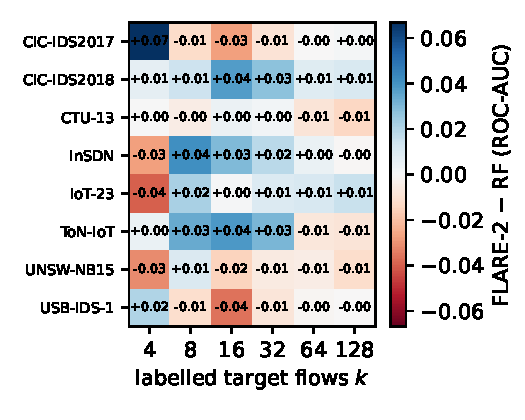
\includegraphics[width=0.55\textwidth]{figures/heatmap.pdf}
\caption{ROC-AUC difference FLARE-2 minus RF per target and $k$.}\label{fig:heat}
\end{figure}

\subsection{Comparison with a tabular foundation model}
Table~\ref{tab:binary} includes TabPFN-3.5.
On seed 0 the mean ROC-AUC over targets and $k$ is 0.862 for TabPFN-3.5, 0.857 for TabPFN-3, 0.850 for FLARE-2 and for target-only CatBoost, 0.846 for RF.
TabPFN-3.5 is higher than FLARE-2 on all 8 targets ($-0.012$ for FLARE-2 minus TabPFN-3.5, $p_{\text{Holm}}=0.016$ over the two versions; TabPFN-3: $-0.008$, $p_{\text{Holm}}=0.016$), and the 3-seed difference to TabPFN-3.5 is $-0.014$ (95\% interval $[-0.018,-0.011]$, 0 of 8 targets in favour of FLARE-2, standard deviation over seeds 0.002; Table~\ref{tab:tabpfn}).
The sign holds for the mean over targets at every $k$ and in both ranges ($k\le16$: $-0.016$; $k\ge32$: $-0.013$ over three seeds), although FLARE-2 is higher on 2 of 8 targets at some single values of $k$.
TabPFN-3.5 is also above the tree ensembles on seed 0 ($+0.016$ over RF on 8 of 8 targets, $+0.012$ over target-only CatBoost on 7 of 8, uncorrected $p=0.008$ and $0.016$; these comparisons were added after the five-baseline family of Table~\ref{tab:stats} was fixed) and not different from source-pretrained CatBoost ($+0.017$, 5 of 8 targets, $p=0.20$).
The differences are small in absolute terms (0.008 to 0.014 on average, 0.006 to 0.024 on individual targets for TabPFN-3.5 over three seeds), but consistent in sign for every target after averaging over $k$, and for every seed.
At $k=4$ all methods but LR and $k$NN are within 0.02 of each other (0.720 for FLARE-2, 0.736 for TabPFN-3.5).
TabPFN reads only the support rows while FLARE-2 additionally ranks features over the unlabelled target rows, so we do not expect the comparison to favour TabPFN: ranking over the support alone costs FLARE-2 only 0.007 ROC-AUC (Sect.~\ref{sec:fewcontrols}).
We do not know why meta-training on five or six real networks is not better than pretraining on a broad synthetic prior, and we have not tested explanations such as model scale, prior breadth or the number of meta-training datasets.

\begin{table}[t]
\centering\small
\caption{FLARE-2 minus TabPFN in binary ROC-AUC, unit = target (8). W/L: targets where FLARE-2 is higher / lower. Seed 0: $p_{\text{Holm}}$ over the two TabPFN versions within each scope. Three seeds: TabPFN-3.5 only, target-averaged over seeds 0--2, exact Wilcoxon $p$ without correction (rows marked 3 seeds). The last column is $p_{\text{Holm}}$ for seed 0 and uncorrected $p$ for three seeds.}\label{tab:tabpfn}
\begin{tabular}{llrrrr}
\toprule
Seeds & Baseline & Mean diff. & 95\% CI & W/L & p$_{\text{Holm}}$ \\
\midrule
mean over k & seed 0, TabPFN-3 & -0.008 & [-0.011, -0.005] & 0/8 & 0.016 \\
 & seed 0, TabPFN-3.5 & -0.012 & [-0.015, -0.009] & 0/8 & 0.016 \\
 & 3 seeds, TabPFN-3.5 & -0.014 & [-0.018, -0.011] & 0/8 & 0.008 \\
\midrule
k$\leq$16 & seed 0, TabPFN-3 & -0.008 & [-0.014, -0.002] & 1/7 & 0.055 \\
 & seed 0, TabPFN-3.5 & -0.014 & [-0.019, -0.009] & 1/7 & 0.031 \\
 & 3 seeds, TabPFN-3.5 & -0.016 & [-0.021, -0.012] & 0/8 & 0.008 \\
\midrule
k$\geq$32 & seed 0, TabPFN-3 & -0.008 & [-0.010, -0.005] & 0/8 & 0.016 \\
 & seed 0, TabPFN-3.5 & -0.010 & [-0.014, -0.007] & 0/8 & 0.016 \\
 & 3 seeds, TabPFN-3.5 & -0.013 & [-0.017, -0.009] & 0/8 & 0.008 \\
\bottomrule
\end{tabular}

\end{table}

\subsection{Attack-class level}
Table~\ref{tab:class} summarises per-class detection (class $c$ against benign, $k$ labelled flows of each) and $N$-way attack-type classification over 57 (target, class) detection tasks.
FLARE-2 has higher per-class ROC-AUC than RF and CatBoost on 7 of 8 targets (mean $+0.014$ and $+0.015$ over targets, $p=0.016$ before correction; the unit-level $p<0.001$ is optimistic because classes within a target are correlated).
It has a lower false-positive rate (by $0.05$; lower on 7 of 8 targets, $p=0.078$ at target level) and a lower recall (by $0.03$ to $0.04$; $p\le0.016$) at the default threshold of 0.5, so part of the ROC-AUC gain is a different operating point and not a free gain in detection.
Repeating the class-level evaluation with meta-training seeds 1 and 2 and averaging each target over the three seeds (Holm-adjusted over the four baselines, unit = target) gives the same picture with firmer tests: per-class ROC-AUC is higher than RF and CatBoost by $+0.011$ on 7 of 8 targets ($p_{\text{Holm}}=0.047$ for both), the false-positive rate is lower on 7 of 8 targets ($p_{\text{Holm}}=0.047$) and recall is lower on all 8 targets ($p_{\text{Holm}}=0.031$), so the operating-point caveat stands.
On $N$-way macro-F1, seed 0 gives $+0.026$ and $+0.022$ over RF and CatBoost (higher on 3 of 8 targets, $p=0.74$) and three seeds $+0.021$ and $+0.018$, which is not significant; FLARE-2 is significantly higher than LR and $k$NN.
$N$-way balanced accuracy, in contrast, is lower than CatBoost by $0.022$ (lower on 7 of 8 targets, $p_{\text{Holm}}=0.047$) and than RF by $0.023$ ($p_{\text{Holm}}=0.078$) over three seeds.
Per-target values are in Table~\ref{tab:classtarget}.

At class level TabPFN-3.5 is not better than FLARE-2 in ranking (Table~\ref{tab:tabpfnclass}): per-class ROC-AUC differs by $-0.002$ (95\% interval $[-0.014,+0.006]$, FLARE-2 higher on 4 of 8 targets) and $N$-way macro-F1 by $-0.014$ ($[-0.049,+0.019]$), neither significant, and the false-positive rate is not different.
TabPFN-3.5 has higher recall at the default threshold (by $0.043$ per class, 0 of 8 targets in favour of FLARE-2, $p_{\text{Holm}}=0.047$) and higher $N$-way balanced accuracy (by $0.048$, $p_{\text{Holm}}=0.078$), which is the same operating-point difference that FLARE-2 shows against the trees.
This comparison is seed 0 only, uses five draws, and, for five targets, a subsample of the query rows.

\begin{table}[t]
\centering\small
\caption{Class-level FLARE-2 minus TabPFN-3.5 (seed 0, $k\le16$ per class, five draws), unit = target (8). W/L: targets where FLARE-2 is higher / lower. $p$: exact Wilcoxon over targets, Holm-adjusted over the five metrics. For FPR a negative difference favours FLARE-2.}\label{tab:tabpfnclass}
\begin{tabular}{lrrrr}
\toprule
Metric & Mean diff. & 95\% CI & W/L & $p$ (Holm) \\
\midrule
Per-class ROC-AUC & -0.002 & [-0.014, +0.006] & 4/4 & 1.000 \\
Per-class FPR & -0.020 & [-0.050, +0.015] & 2/6 & 0.938 \\
Per-class recall & -0.043 & [-0.061, -0.025] & 0/8 & 0.047 \\
$N$-way macro-F1 & -0.014 & [-0.049, +0.019] & 3/5 & 1.000 \\
$N$-way balanced accuracy & -0.048 & [-0.070, -0.026] & 1/7 & 0.078 \\
\bottomrule
\end{tabular}

\end{table}

\begin{table}[t]
\centering\scriptsize
\caption{Class-level differences, FLARE-2 minus baseline. ``targets'': mean over the 8 targets of the target mean, count of targets where FLARE-2 is higher, exact Wilcoxon $p$ over targets (uncorrected). ``units'': mean over (target, class) pairs, $k\in\{2,4,8,16\}$ labelled flows per class. For FPR a negative difference favours FLARE-2.}\label{tab:class}
\begin{tabular}{llccccc}
\toprule
Metric & Baseline & $\Delta$ (targets) & FLARE-2 higher & $p$ & $\Delta$ (units) & units \\
\midrule
Per-class ROC-AUC & RF & +0.014 & 7/8 & 0.016 & +0.012 & 57 \\
Per-class ROC-AUC & CatBoost & +0.015 & 7/8 & 0.016 & +0.013 & 57 \\
Per-class ROC-AUC & LR & +0.082 & 8/8 & 0.008 & +0.075 & 57 \\
Per-class ROC-AUC & kNN & +0.175 & 8/8 & 0.008 & +0.167 & 57 \\
Per-class recall@0.5 & RF & -0.041 & 0/8 & 0.008 & -0.044 & 57 \\
Per-class recall@0.5 & CatBoost & -0.026 & 1/8 & 0.016 & -0.030 & 57 \\
Per-class recall@0.5 & LR & -0.025 & 2/8 & 0.078 & -0.030 & 57 \\
Per-class recall@0.5 & kNN & -0.048 & 1/8 & 0.023 & -0.056 & 57 \\
Per-class FPR@0.5 & RF & -0.053 & 1/8 & 0.078 & -0.052 & 57 \\
Per-class FPR@0.5 & CatBoost & -0.052 & 1/8 & 0.078 & -0.050 & 57 \\
Per-class FPR@0.5 & LR & -0.077 & 1/8 & 0.016 & -0.074 & 57 \\
Per-class FPR@0.5 & kNN & -0.334 & 0/8 & 0.008 & -0.330 & 57 \\
N-way macro-F1 & RF & +0.026 & 3/8 & 0.742 & +0.026 & 8 \\
N-way macro-F1 & CatBoost & +0.022 & 3/8 & 0.742 & +0.022 & 8 \\
N-way macro-F1 & LR & +0.074 & 7/8 & 0.016 & +0.074 & 8 \\
N-way macro-F1 & kNN & +0.127 & 8/8 & 0.008 & +0.127 & 8 \\
\bottomrule
\end{tabular}

\end{table}

\begin{table}[t]
\centering\small
\caption{Per-target class-level results. Left: per-class ROC-AUC at $k=4$ per class. Right: $N$-way macro-F1 at $k=16$ per class. InSDN is omitted because it has no class-level evaluation at $k=16$.}\label{tab:classtarget}
\begin{tabular}{lcccccc}
\toprule
& \multicolumn{3}{c}{Per-class ROC-AUC, $k{=}4$} & \multicolumn{3}{c}{N-way macro-F1, $k{=}16$} \\
\cmidrule(lr){2-4}\cmidrule(lr){5-7}
Target & F2 & RF & CB & F2 & RF & CB \\
\midrule
CIC-IDS2017 & \textbf{0.957} & 0.942 & 0.949 & \textbf{0.504} & 0.456 & 0.448 \\
CIC-IDS2018 & \textbf{0.889} & 0.879 & 0.875 & \textbf{0.658} & 0.517 & 0.582 \\
CTU-13 & \textbf{0.863} & 0.853 & 0.852 & \textbf{0.299} & 0.329 & 0.350 \\
IoT-23 & \textbf{0.879} & 0.842 & 0.841 & \textbf{0.644} & 0.562 & 0.589 \\
ToN-IoT & \textbf{0.927} & 0.906 & 0.925 & \textbf{0.680} & 0.705 & 0.688 \\
UNSW-NB15 & \textbf{0.857} & 0.845 & 0.839 & \textbf{0.294} & 0.337 & 0.323 \\
USB-IDS-1 & \textbf{0.995} & 0.998 & 0.999 & \textbf{0.461} & 0.461 & 0.468 \\
\bottomrule
\end{tabular}

\end{table}

\subsection{Ablations and controls}\label{sec:ablation}
We retrain FLARE-2 with one component changed and evaluate on the same support draws as the main results (checked: the RF baseline reproduces the earlier numbers exactly).
This costs one training run per cell, so we use a single meta-training seed and two targets (CTU-13 and CIC-IDS2017).
The study therefore shows direction, not significance.

\begin{table}[t]
\centering\small
\caption{Ablations, seed 0, 10 support draws per $k$ for binary metrics; class-level metrics use 10 draws for the no-permutation, in-source and CIC-IDS2017 loss-mask rows and 5 for the others. Binary ROC-AUC at $k\in\{4,16,64\}$, $N$-way macro-F1 at $k{=}16$ per class, and per-class ROC-AUC at $k{=}4$. Rows are compared with their own reference: the first three rows with FLARE-2, the last two with the loss-masked model.}\label{tab:ablation}
\resizebox{\linewidth}{!}{\begin{tabular}{lrrrrrrrrrr}
\toprule
 & \multicolumn{5}{c}{CTU-13} & \multicolumn{5}{c}{CIC-IDS2017} \\
Variant & $k{=}4$ & $k{=}16$ & $k{=}64$ & F1@16 & AUC@4 & $k{=}4$ & $k{=}16$ & $k{=}64$ & F1@16 & AUC@4 \\
\midrule
FLARE-2 & 0.599 & 0.704 & 0.797 & 0.299 & 0.863 & 0.785 & 0.861 & 0.965 & 0.504 & 0.957 \\
No slot perm. & 0.615 & 0.714 & 0.788 & 0.300 & 0.867 & 0.709 & 0.368 & 0.942 & 0.567 & 0.957 \\
In-source val. & 0.604 & 0.703 & 0.794 & 0.310 & 0.862 & 0.784 & 0.870 & 0.965 & 0.562 & 0.959 \\
Loss mask & 0.594 & 0.707 & 0.792 & 0.312 & 0.863 & 0.775 & 0.890 & 0.969 & 0.582 & 0.963 \\
Loss mask, binary & 0.563 & 0.671 & 0.779 & 0.268 & 0.858 & 0.776 & 0.856 & 0.949 & 0.566 & 0.959 \\
\bottomrule
\end{tabular}
}
\end{table}

Table~\ref{tab:ablation} shows four things.
\emph{Slot permutation.} Removing the random class-to-slot assignment matches FLARE-2 on CTU-13 (differences of at most 0.018 AUC over all $k$) but is unstable on CIC-IDS2017: binary AUC at $k{=}16$ falls to 0.368 and is below 0.5 in most draws at $k{=}8$ and $k{=}16$ (6 of 10 and 8 of 10 draws), while $k{=}64$ recovers to 0.942, still 0.023 below FLARE-2; its $N$-way macro-F1 at $k{=}16$ is not lower (0.567 against 0.504).
A diagnostic on CIC-IDS2017 at $k{=}16$ (6 draws) explains the inversion: the model trained without permutation uses the index of the label slot as a cue about the class. With the benign class in slot 0 it scores 0.443; with the two class ids swapped it scores 0.883, equal to the loss-masked model with random slots (0.882 in both orientations, as a class-equivariant model must). The ranking is therefore inverted by the orientation of the slots, not by noise, and random slot assignment removes this dependence.
\emph{Validation.} Selecting the checkpoint on in-source validation episodes instead of a held-out source changes binary AUC by at most 0.009 at $k\in\{4,16,64\}$ on both targets, by $+0.048$ at $k{=}8$ on CIC-IDS2017 (0.842 against 0.794) and raises $N$-way macro-F1 at $k{=}16$ on CIC-IDS2017 (0.562 against 0.504), so we cannot show that held-out validation matters on these two targets.
\emph{Loss mask.} Masking queries without support gives similar binary AUC on CTU-13 and higher AUC at $k{\ge}16$ on CIC-IDS2017 (0.890 against 0.861 at $k{=}16$), with higher $N$-way macro-F1 on both targets. Trained on all eight targets (seed 0), the masked model has mean binary ROC-AUC 0.851 against 0.850 for FLARE-2, with per-target differences from $-0.010$ (InSDN) to $+0.019$ (CIC-IDS2018) and a gain on 4 of 8 targets, so the CIC-IDS2017 gain is not a general effect.
\emph{Class-level tasks.} Training on binary tasks only lowers binary AUC on CTU-13 by 0.01 to 0.04 and on CIC-IDS2017 by 0.01 to 0.05 at $k{\ge}16$, and lowers $N$-way macro-F1 at $k{=}16$ on both targets (0.268 against 0.312 on CTU-13, 0.566 against 0.582 on CIC-IDS2017), while the per-class AUC at $k{=}4$ is nearly unchanged (0.858 against 0.863 and 0.959 against 0.963).
Class-level tasks help binary AUC modestly (0.01 to 0.05); their effect on $N$-way macro-F1 ($-0.044$ on CTU-13 and $-0.016$ on CIC-IDS2017 for binary-only training, relative to the loss-masked model) is within the spread between other variants on CIC-IDS2017 (0.504 to 0.582), and we find no evidence that they drive per-class ranking.

\subsubsection{Controls}\label{sec:fewcontrols}
These controls use the meta-training seed 1 models of all eight targets and the same support draws for every variant.

\paragraph{Does the transductive normalisation matter?}
The default ranks each feature over the support and all query rows of the target. Ranking over the support and a random subsample of 256 query rows, the size seen in meta-training, gives the same mean binary ROC-AUC (0.847 against 0.847; per-target differences between $-0.003$ and $+0.003$). Ranking over the support alone, with queries mapped through the support distribution, lowers it by 0.007 on average (lower on 6 of 8 targets, by up to 0.017). The use of unlabelled target rows therefore has a small effect, and the 256-row reference removes the dependence on the full test split.

\paragraph{Does the model read the rule from the support labels?}
At $k{=}16$ and $k{=}64$ (5 draws), permuting the support labels among the support rows gives ROC-AUC between 0.41 and 0.69 on the individual targets (mean 0.54 at $k{=}16$, 0.51 at $k{=}64$; three targets fall below 0.5 at each $k$), against 0.82 and 0.91 with the true labels. Using the support rows of another draw of the same target gives 0.81 and 0.91, so the model reads the rule from labelled rows of the target and not from the particular rows. Swapping the two class ids leaves the AUC unchanged, as expected for a class-equivariant readout. We did not test support sets from a different target.

\section{Discussion, limitations and conclusion}\label{sec:disc}
\subsection{Discussion}
The benchmark shows that cross-dataset transfer fails on average with every method we ran, though not on every pair: three to five pairs exceed 0.8 per tree method, mostly with USB-IDS-1 as source or target.
It is not repaired by the usual remedies: default-setting tuning on the pair we tested, normalisation, feature selection, alignment, adversarial invariance, prior correction and self-training, and RIFT is not rescued by the true prior or a truly benign anchor.
Below-chance ROC-AUC on 36 to 48\% of the pairs (21 to 29\% below 0.40) for the tree ensembles is what an inverted rule would produce, but also what a different attack mix would produce; the single-family transfer, with the attack mix held fixed up to the family, is also near chance (median 0.545), which excludes attack mix alone.
What remains is a difference in benign traffic, in how flows are measured, or in the conditional label distribution, and the controls cannot tell which.

\paragraph{What the evidence does not show.}
First, the per-feature sign flips arise when the attack mix differs, even without a labelling disagreement, and we have no within-dataset null for them.
The nearest-neighbour test conditions on flow statistics but is restricted to the overlap region, which is small for most pairs (a median overlap fraction below 0.01), and a $\kappa$ near zero there means only that the neighbours' labels are uninformative; three of the 19 values are exactly zero.
Second, ``labelling function'' is not the right name for what the benchmark can establish: with only 13 flow features and no ports, flags or payload, $P(y\mid x)$ also changes when relevant variables are omitted and their distribution differs between datasets, even if every dataset applied the same rule.
The datasets label attacks by different procedures (attacker address and schedule, scenario, tool logs), which we did not tabulate.
Third, the oracle control covers one informative pair, and the single-family control uses a coarse family assignment and cannot separate benign and measurement differences from the conditional label distribution.
Fourth, the seven datasets are public laboratory captures with their own labelling errors \citep{engelen2021troubleshooting}, the flow features come from different extractors whose byte and duration semantics are not audited here, and the distinct-row sampling changes attack priors relative to natural traffic; the features and sampling are not varied.
Fifth, RIFT is one design; the negative result concerns this design and these ablations, and the baselines run with default settings.

\paragraph{Implications.}
Evaluation should report cross-dataset results with a pair taxonomy and per-pair distributions, because same-laboratory pairs can be the worst, one favourable pair hides the rest, and a mean of values near 0.2 and 0.97 says little; a method should be compared with its own baseline in the same setting, as here, because it can otherwise look useful for the wrong reason.
Methods that assume a fixed $P(y\mid x)$ should not be expected to repair these transfers, and the few-label results suggest that a few labelled flows of the target network are worth more than the source data on average, for the model family we tested.

\paragraph{Few-label transfer.}
The few-label study (Sect.~\ref{sec:fewlabel}) adds three observations.
FLARE-2 is not distinguishable from fixed-setting tree ensembles on binary ROC-AUC, and a general-purpose tabular foundation model (TabPFN versions 3 and 3.5, without any training or tuning on network data by us) is better than both on every target, by a small but consistent margin of 0.008 to 0.014 ROC-AUC on average.
At attack-class level FLARE-2 ranks classes slightly better than the trees (per-class ROC-AUC $+0.011$ over three seeds) but with lower recall at the default threshold, and TabPFN-3.5 ranks them as well as FLARE-2 with higher recall.
The source datasets therefore help the few-label setting only through a pretrained prior, and meta-training that prior on a handful of real networks did not improve on a prior pretrained on synthetic tasks in our experiments; whether more networks, more steps or a larger model would change this is untested.

\subsection{Limitations of the few-label study}
\begin{itemize}
\item The main tables and figures use meta-training seed 0 with 10 support draws per target; seeds 1 and 2 were run for all targets and are summarised in Table~\ref{tab:seeds} and in the text for the class level (the class-level tables themselves are seed 0), and the ablations use one seed and two targets (the loss-mask comparison uses all eight targets, the controls the seed-1 models).
\item FLARE-2 is not better than fixed-setting tree ensembles on binary ROC-AUC, and TabPFN is better than FLARE-2 on every target; its remaining gains are class-level and conditional on the operating point.
\item The class-level TabPFN comparison is seed 0 only, with five draws and, for five of the eight targets, a stratified subsample of at most 5\,000 query rows per task (checked on one target: differences of at most 0.005).
\item The TabPFN comparison uses default settings, three seeds for version 3.5 and one for version 3, and the released weights under a non-commercial license; a tuned or fine-tuned TabPFN, or a tuned FLARE-2, could change the gaps, which are 0.008 to 0.014 ROC-AUC on average.
\item Eight datasets from five laboratories (UNB, Sannio, UCD, UNSW, CTU), so datasets are not independent units; results on other networks may differ.
\item FLARE-2 normalises features by rank over the unlabelled target rows it scores, which is transductive in the target features (a 256-row query reference gives the same ROC-AUC and support-only ranks lower it by 0.007, Sect.~\ref{sec:fewcontrols}), and the baselines get no such information; one meta-trained model per target is needed (leave-one-dataset-out), and each model sees only five or six training datasets. All eight targets were used while choosing the architecture and the task mix, so there is no untouched test set. Source-pretrained CatBoost is better than FLARE-2 at $k=4$ on four targets.
\item Queries whose class has no support row (label noise at $k=1$) receive a target logit of $-10^{9}$. This produced training losses of order $10^{6}$ and, in one binary-only ablation run, made validation loss pick a collapsed checkpoint (AUC about 0.50); checkpoint selection now scores supported queries only. The checkpoint selection of the main FLARE-2 runs is unaffected (their validation episodes contained no unsupported queries), but their training loss includes these queries (logged loss of order $10^{6}$ to $10^{7}$). The loss-masked variant, trained on all eight targets with seed 0, has mean binary ROC-AUC 0.851 against 0.850 for FLARE-2, with per-target differences between $-0.010$ and $+0.019$ and a gain on 4 of 8 targets (Sect.~\ref{sec:ablation}).
\item Flows only; payload features and temporal context are not used.
\item The datasets are public laboratory captures with their own labelling errors \citep{engelen2021troubleshooting}.
\end{itemize}

\subsection{Conclusion}
On seven public datasets, flow classifiers that reach 0.985 ROC-AUC in-domain reach 0.54 to 0.57 across datasets, with about 40\% of the transfers below chance for the tree ensembles, and transfer within a laboratory is on average worse than across laboratories.
A domain-invariant method designed for the covariate and label shifts of this setting (RIFT) is below its own baseline, and neither the true target prior nor a truly benign anchor makes it better than no adaptation.
Transfer of a single attack family between datasets is also near chance, so a difference of attack mix alone does not explain the failure; the controls are consistent with differences in benign traffic, measurement and the conditional label distribution, which they cannot separate.
What the other datasets can still provide is a prior over how to learn a rule from a few labelled flows.
FLARE-2, a transformer meta-trained on real network tasks, matches fixed-setting tree ensembles on binary detection without fitting the network to the target and modestly improves per-class ranking over the trees (but not over TabPFN-3.5, which also has higher recall), while a general tabular foundation model, TabPFN versions 3 and 3.5, is better on every target (mean over $k$) by 0.008 (version 3, seed 0) to 0.014 (version 3.5, three seeds) ROC-AUC without any training or tuning on network data by us.
The practical conclusion is that labelled flows from the target network, read by a strong pretrained prior, are what works, and that in our experiments meta-training on a handful of real networks did not improve on that prior.
Open problems are the gap to full-label training (0.95--1.00 ROC-AUC) at small $k$, tuning and fine-tuning the foundation model, per-attack-type analysis across laboratories, and testing whether a meta-trainer with more networks, more steps or a larger model closes the gap.

\paragraph{Reproducibility.}
The package, configurations, sampled-row hashes and every raw per-run result are in \url{https://github.com/vinhqdang/cross_ids}. Tables and figures are generated from the result files by the repository scripts.

\bibliographystyle{plainnat}
\bibliography{refs}
\end{document}
